\chapter{Thiết kế hệ thống phân loại tự động}
\paragraph{Giới thiệu} Về nội dung chương này, chúng em sẽ miêu tả lại quá trình mà chúng em đã thiết kế nên hệ thống gồm các bước như cách áp dụng một số design pattern vào việc xây dựng hệ thống, các phác thảo sơ khai của giao diện, cách kết hợp các thư viện lập trình đã giới thiệu với Vaadin Framework và cuối cùng là thiết kế một ontology dùng để trình bày tính năng phân loại sau khi hệ thống được xây dựng thành công.
\section{Giải thích về việc lựa chọn nền tảng sử dụng}
Như đã được trình bày ở mục trên, Vaadin Framework là một nền tảng xây dựng Web dựa trên ngôn ngữ Java, nhưng không giống với phần lớn các framework Web khác vốn hoạt động theo mô hình Model-View-Controller (MVC). Vaadin chỉ cung cấp một bộ gồm rất nhiều UI Component có sẵn (đã được giải thích ở mục trước) làm cho việc xây dựng giao diện được đơn giản hóa một cách tối đa. Vì thế, lập trình viên sẽ không cần phải quan tâm nhiều đến HTML, JavaScript và ít phải quan tâm đến CSS, điều này giúp tập trung vào việc xây dựng logic của hệ thống tốt hơn. Việc thiết kế cho hệ thống này trên nền web sẽ tương tự như khi thiết kế một ứng dụng GUI trên nên Desktop nhờ có Vaadin.
\section{Thiết kế Use Case của hệ thống}
Trước tiên, chúng em xin giới thiệu một cách tổng quan về hoạt động của hệ thống.
 \begin{figure}[ht!]
 	\centering
 	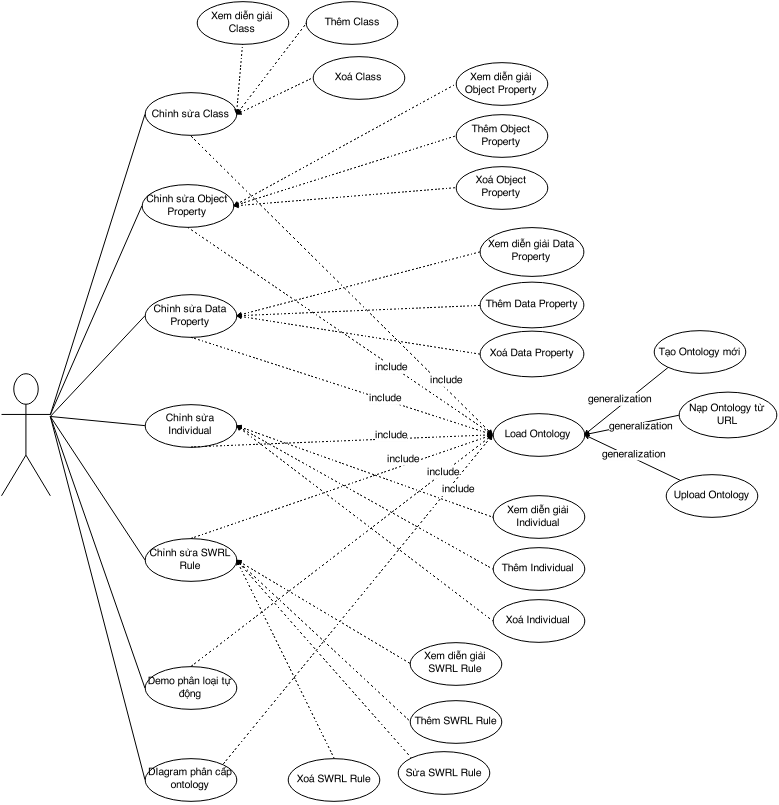
\includegraphics[width=155mm,height=170mm]{Figures/usecase.png}
 	\caption{Sơ đồ Use Case của hệ thống \label{overflow}}
 \end{figure}
\section{Thiết kế giao diện phác thảo}
Hệ thống hay ứng dụng sẽ gồm 2 view chính: view đầu tiên tạm gọi là EntryView dùng để nạp/tạo mới các tài liệu OWL 2. View thứ hai là view chính của ứng dụng, gọi là MainView cho phép thực hiện việc chỉnh sửa ontology, thực hiện suy luận (phục vụ cho tính năng phân loại tự động). 
\begin{figure}[ht!]
	\centering
	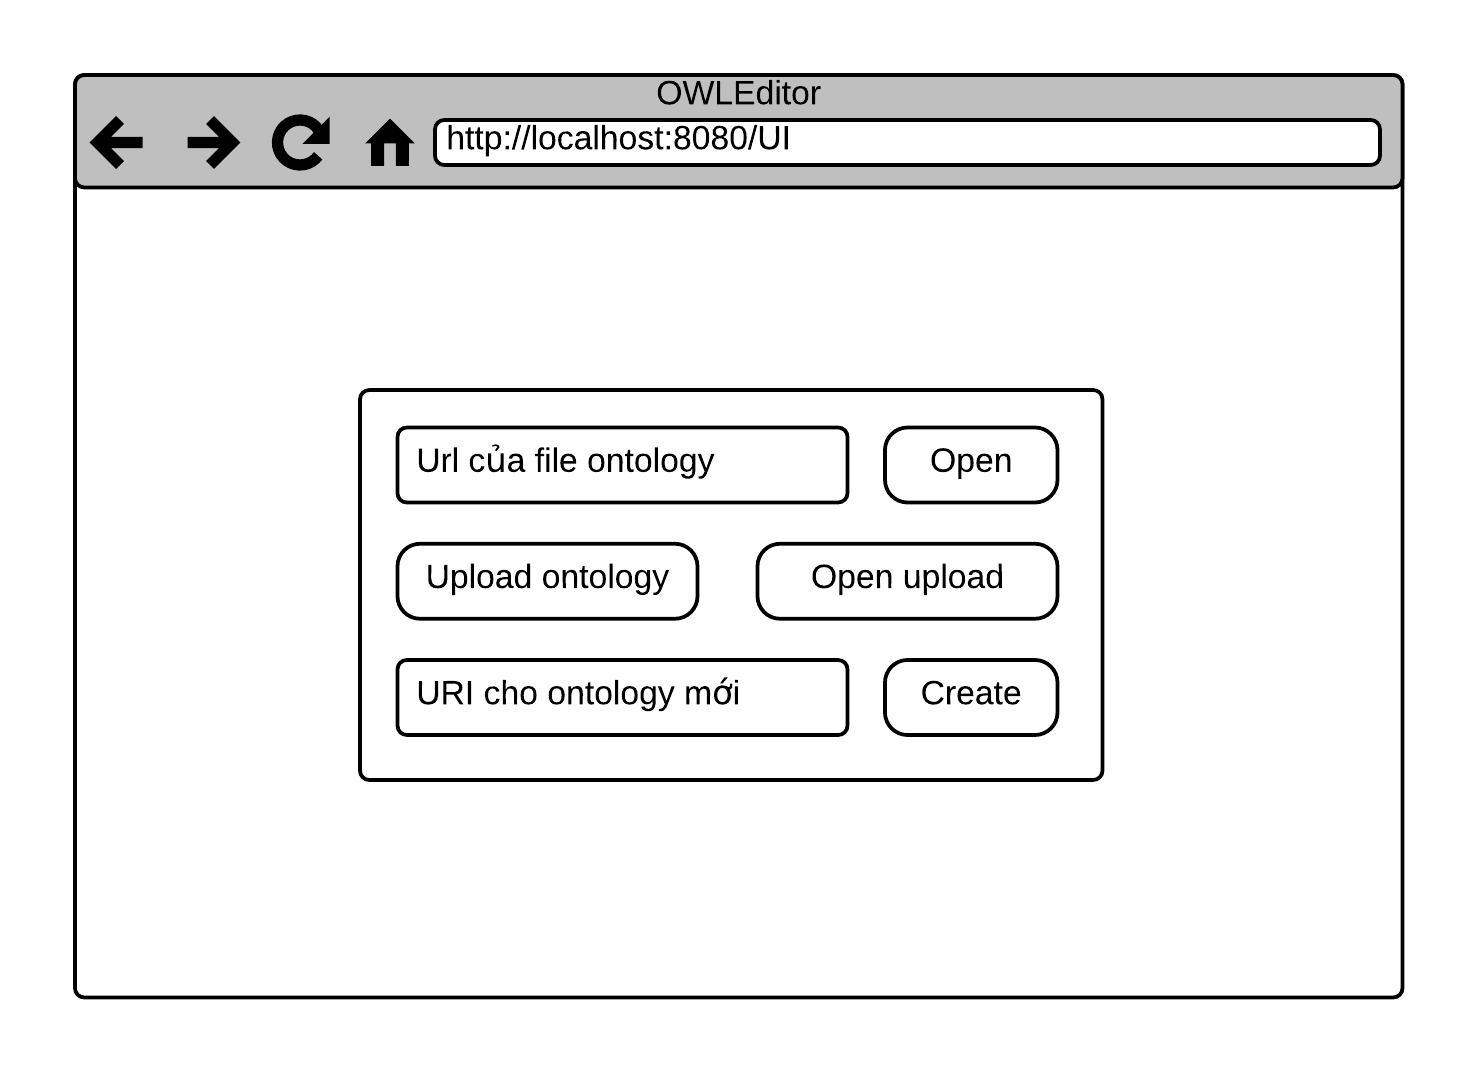
\includegraphics[width=150mm,height=95mm]{Figures/ui_entryview.png}
	\caption{Phác thảo Entry View \label{overflow}}
\end{figure}
MainView sẽ gồm nhiều tab, mỗi loại thực thể (gồm lớp, thuộc tính đối tượng, thuộc tính dữ liệu, cá thể) và SWRL Rule sẽ được tổ chức thành từng tab với tên tương ứng. Ngoài ra, còn có thêm 2 tab khác là tab Demo (demo tính năng phân loại tự động) và tab Diagram (sơ đồ phân cấp các thực thể của Ontology).
\begin{figure}[h!]
	\centering
	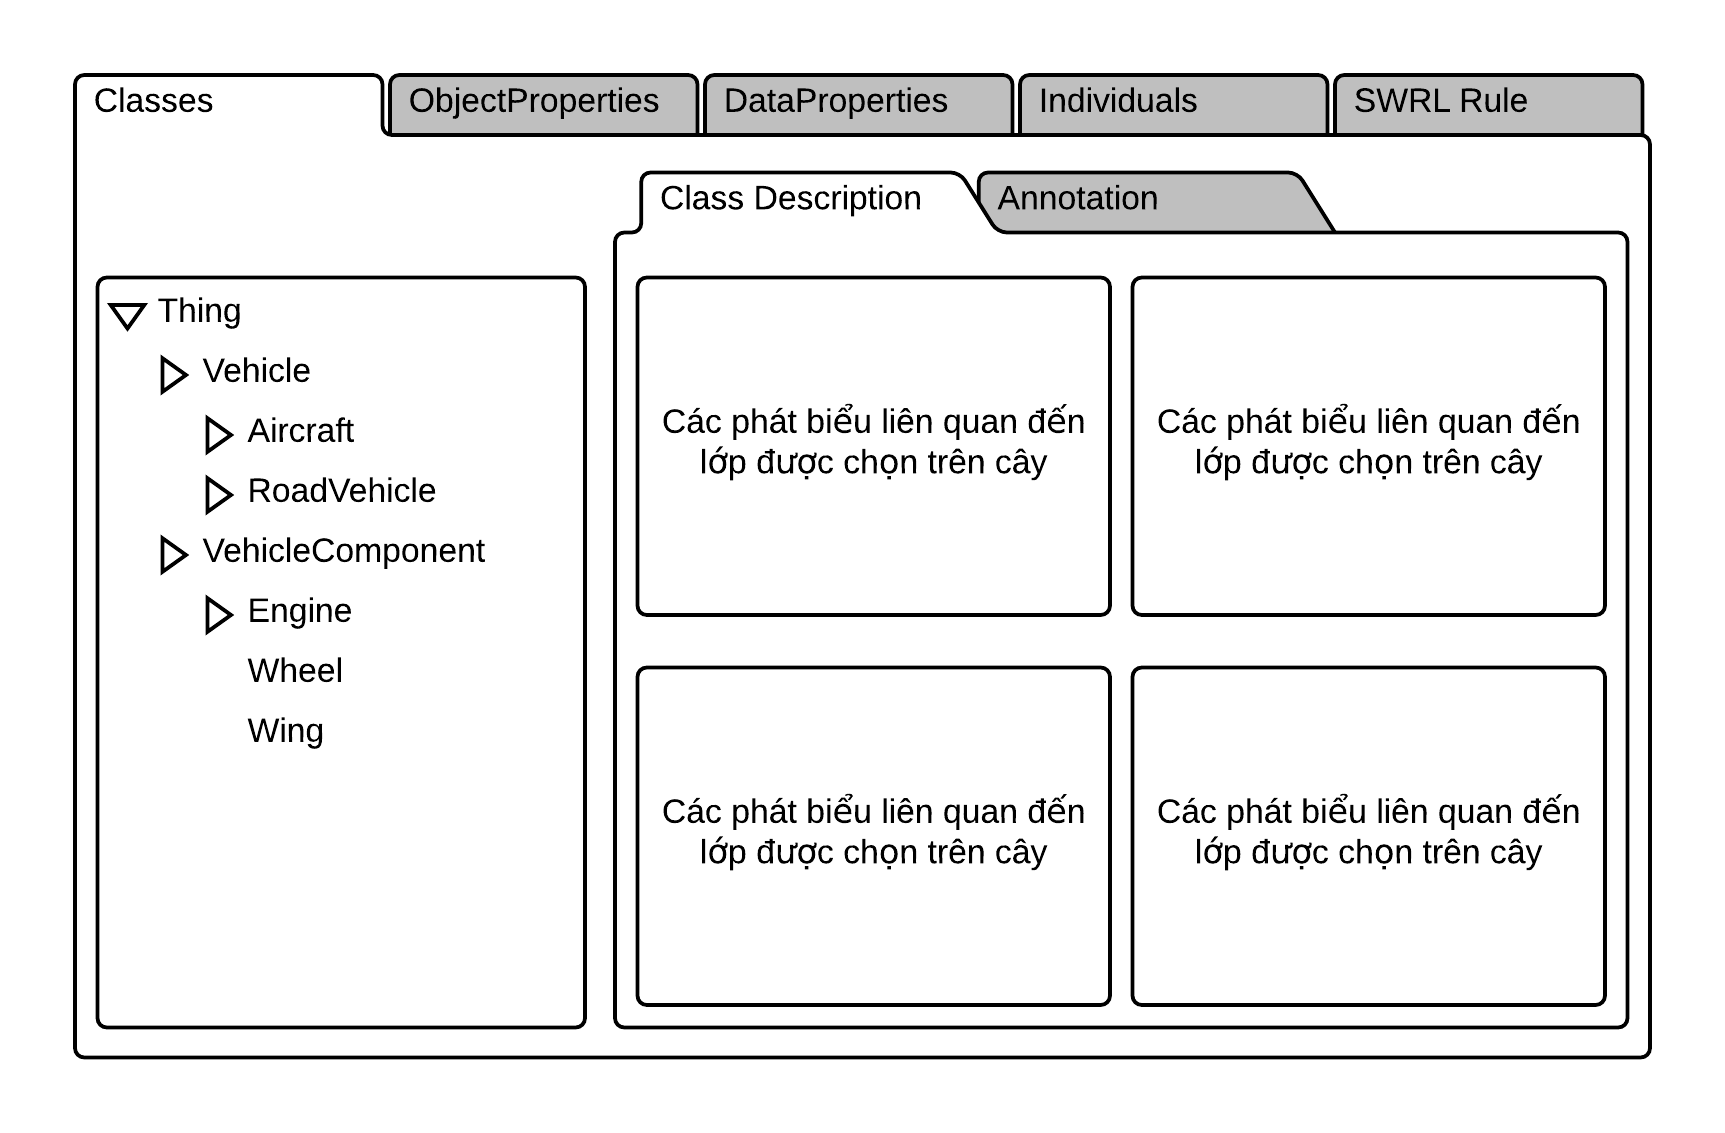
\includegraphics[width=150mm,height=95mm]{Figures/ui_mainview.png}
	\caption{Phác thảo Main View - Tab "Classes" (chứa lớp và các mô tả lớp liên quan) \label{overflow}}
\end{figure}
\begin{figure}[h!]
	\centering
	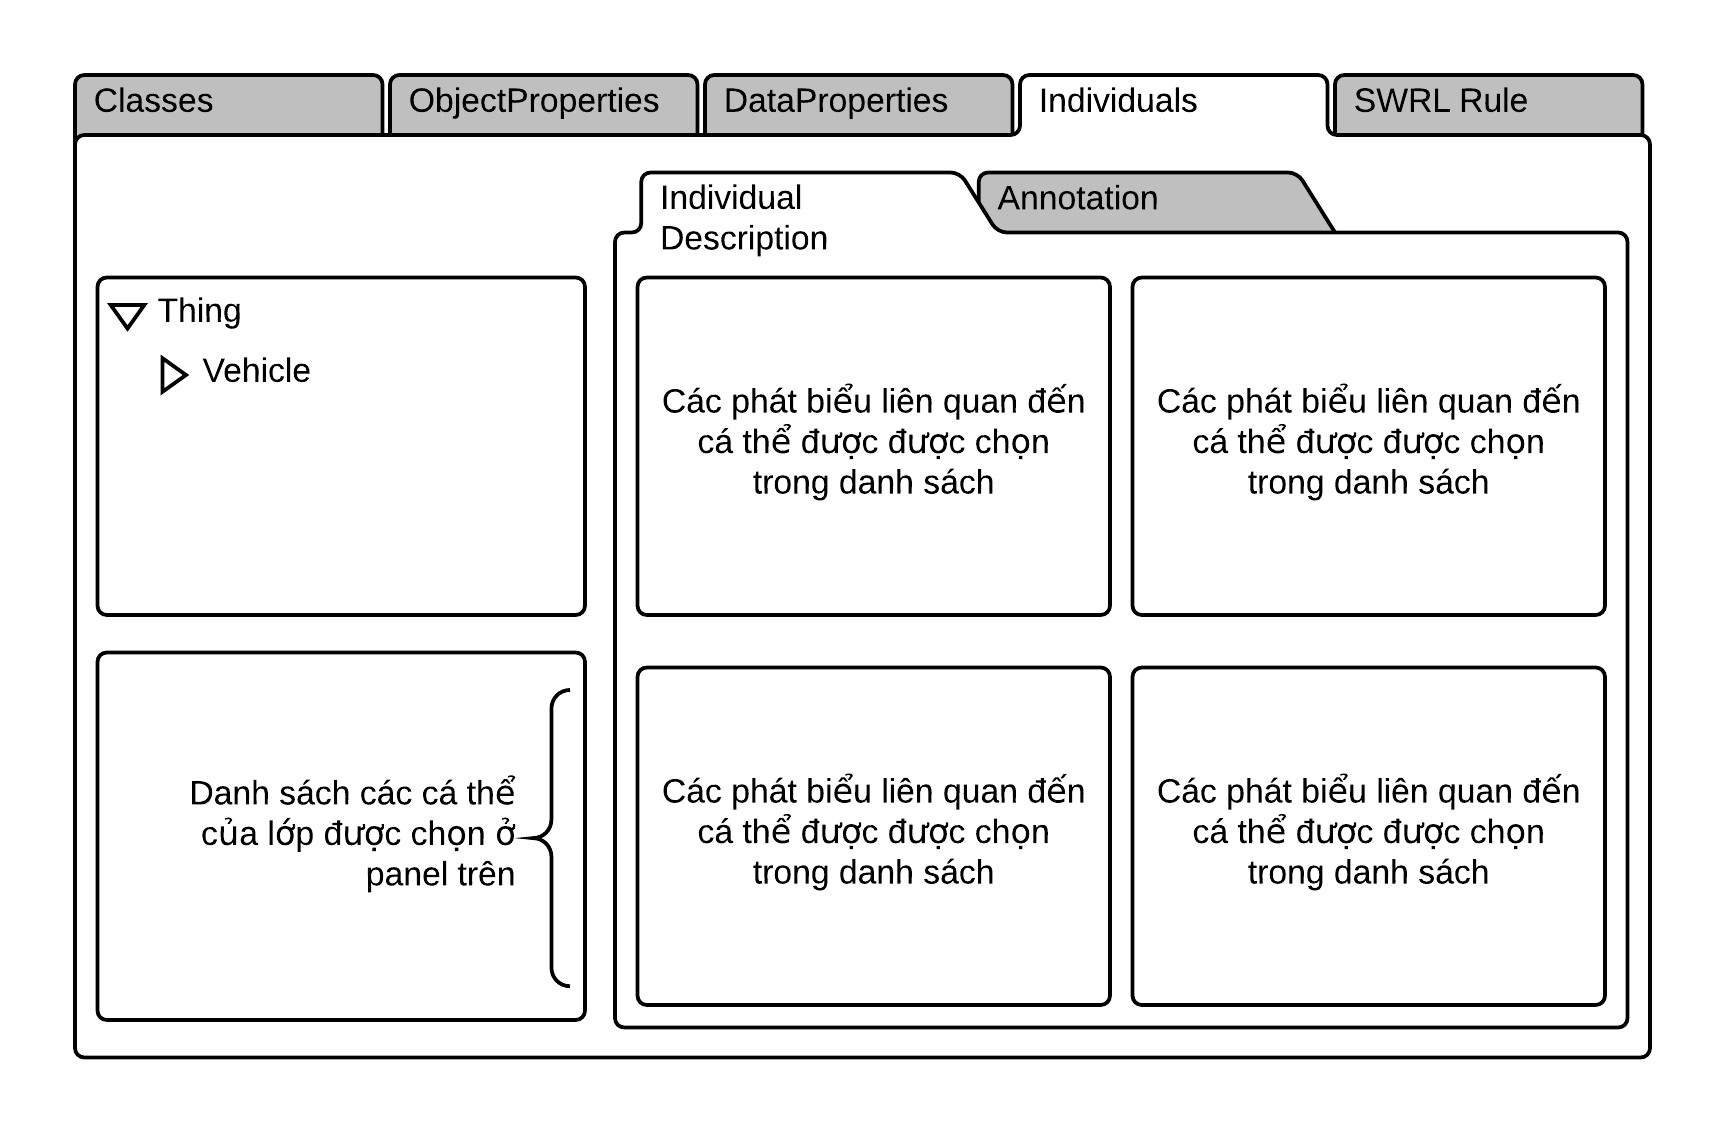
\includegraphics[width=150mm,height=95mm]{Figures/ui_mainview_individual.png}
	\caption{Phác thảo Main View - Tab "Individuals" (chứa cá thể và các mô tả liên quan) \label{overflow}}
\end{figure}
\begin{figure}[h!]
	\centering
	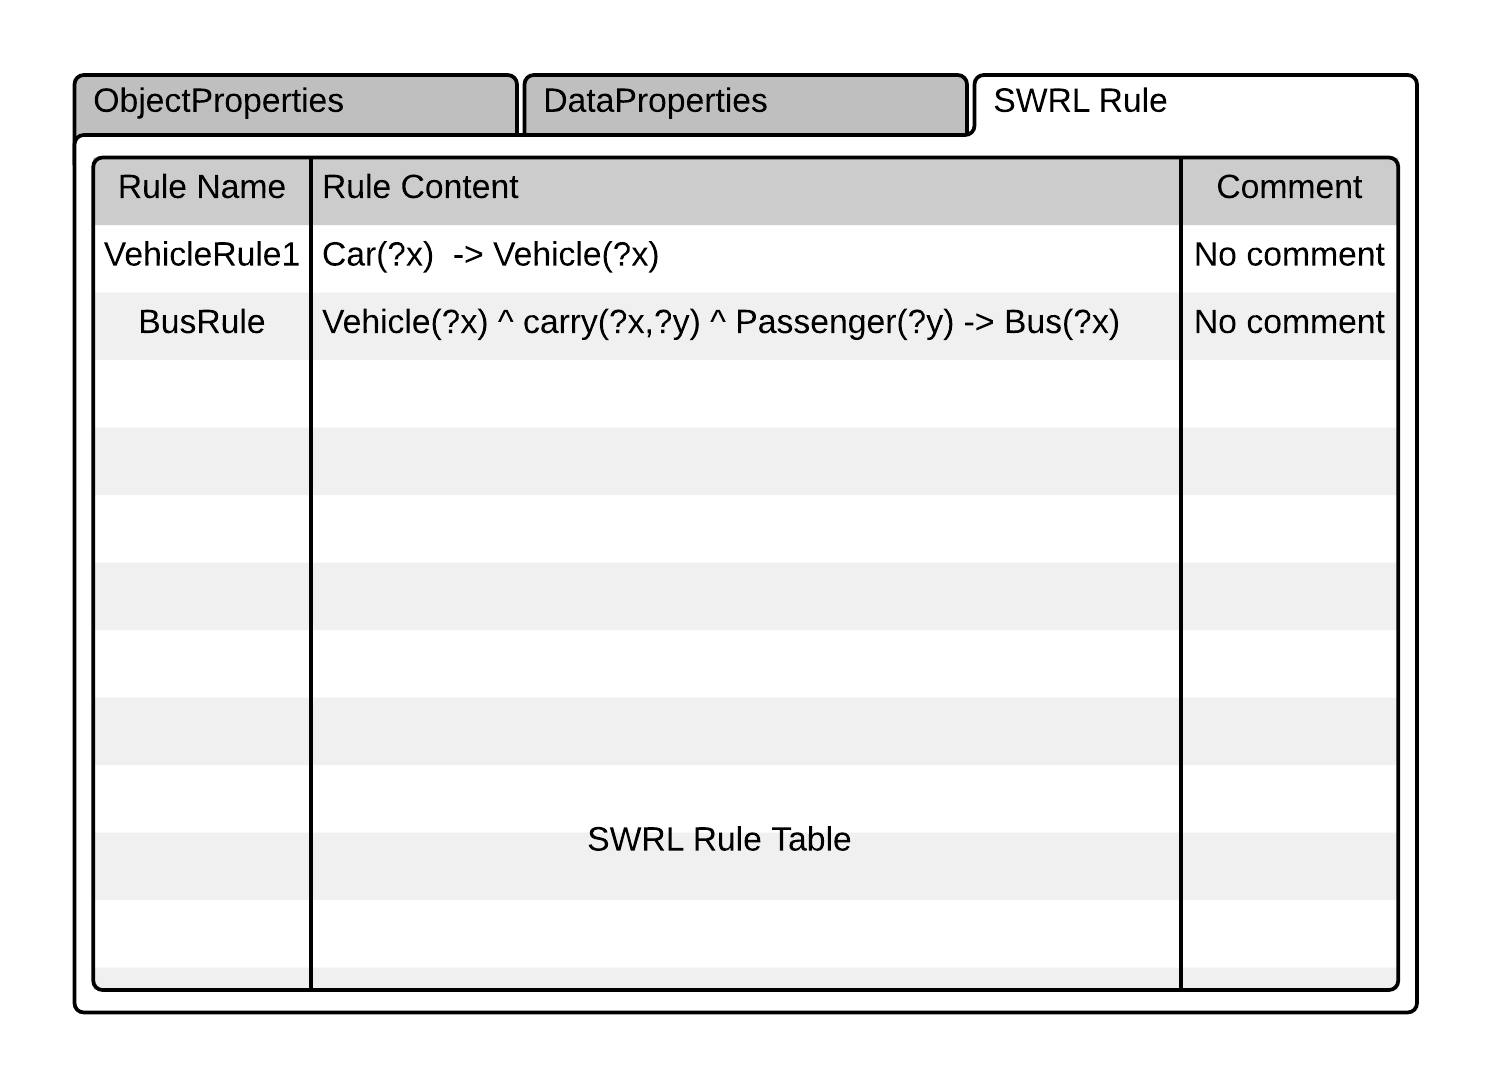
\includegraphics[width=150mm,height=95mm]{Figures/ui_mainview_swrltab.png}
	\caption{Phác thảo Main View - Tab "SWRL Rules" \label{overflow}}
\end{figure}

\begin{figure}[h!]
	\centering
	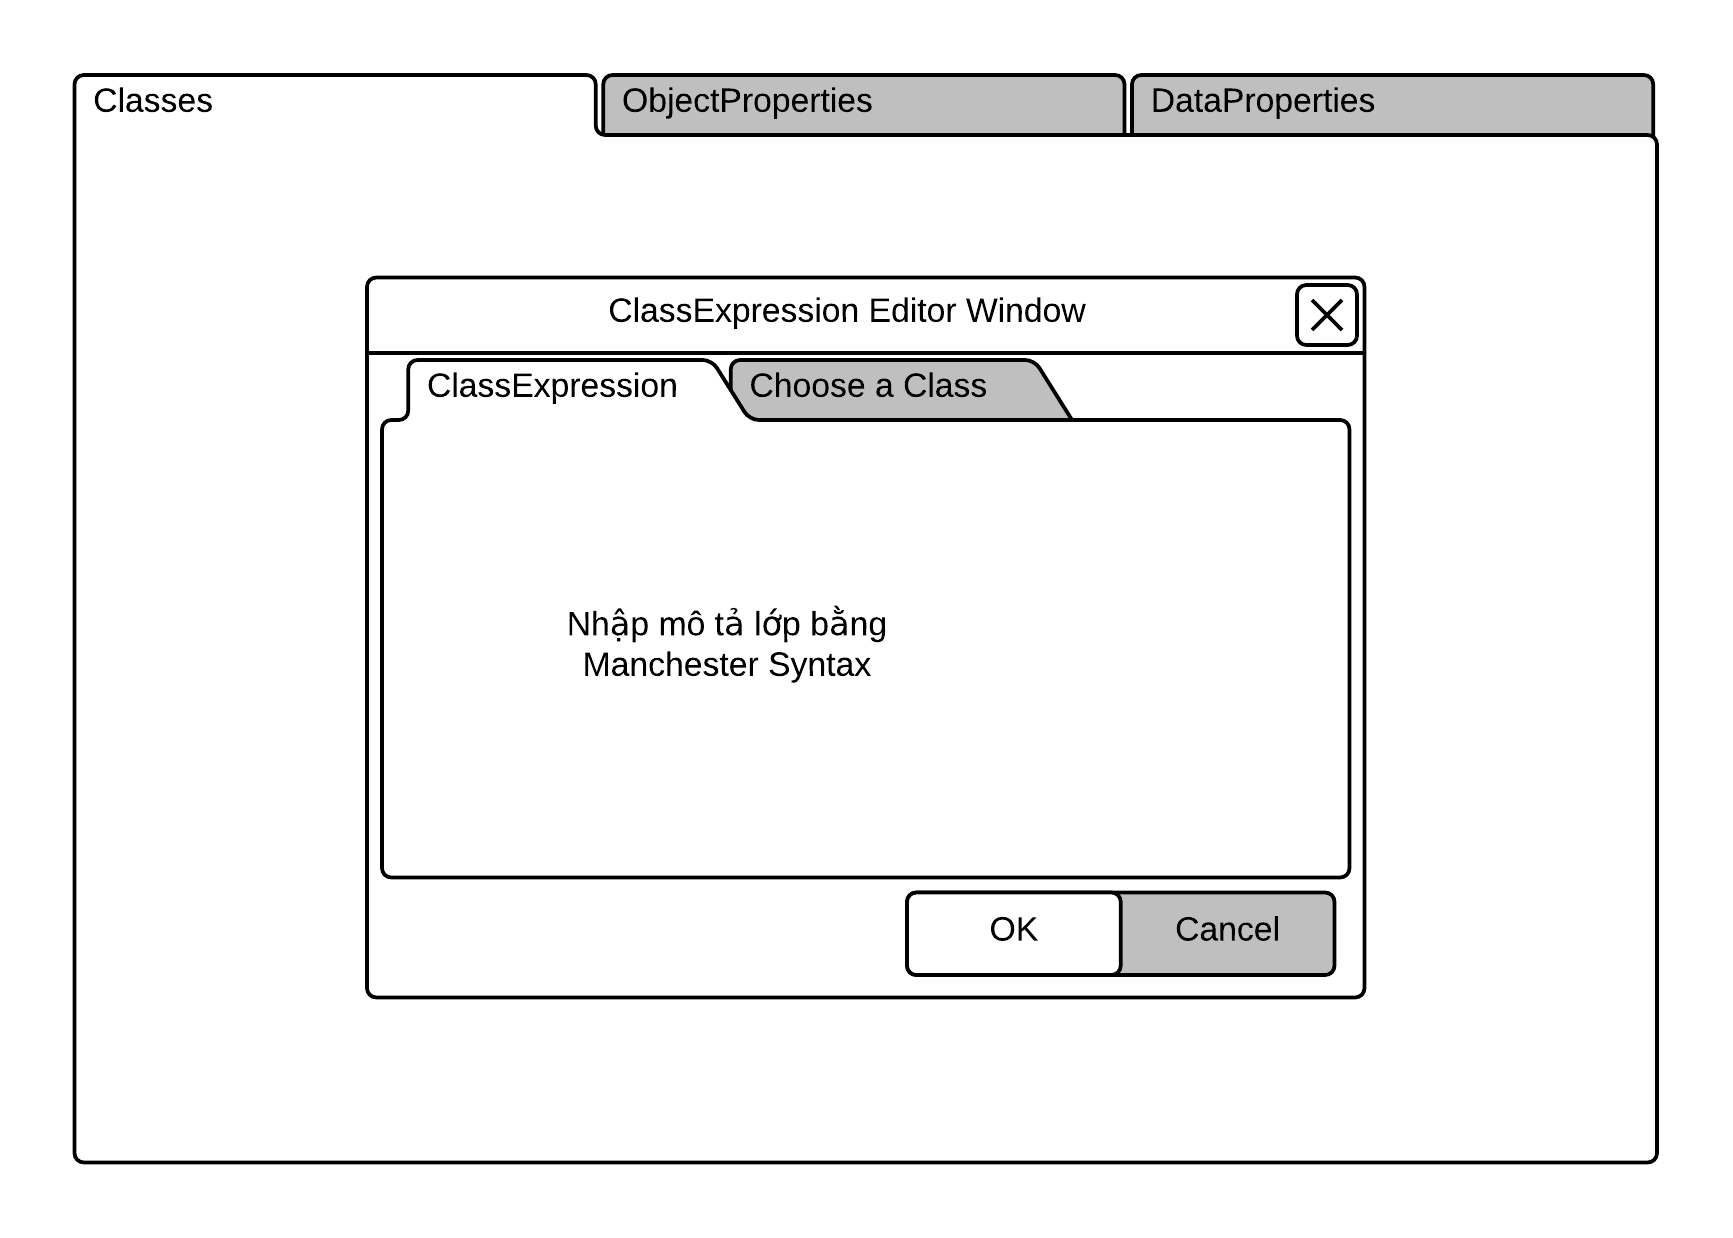
\includegraphics[width=150mm,height=100mm]{Figures/ui_classexpressioneditor.png}
	\caption{Phác thảo cửa sổ biên tập mô tả lớp\label{overflow}}
\end{figure}
\begin{figure}[h!]
	\centering
	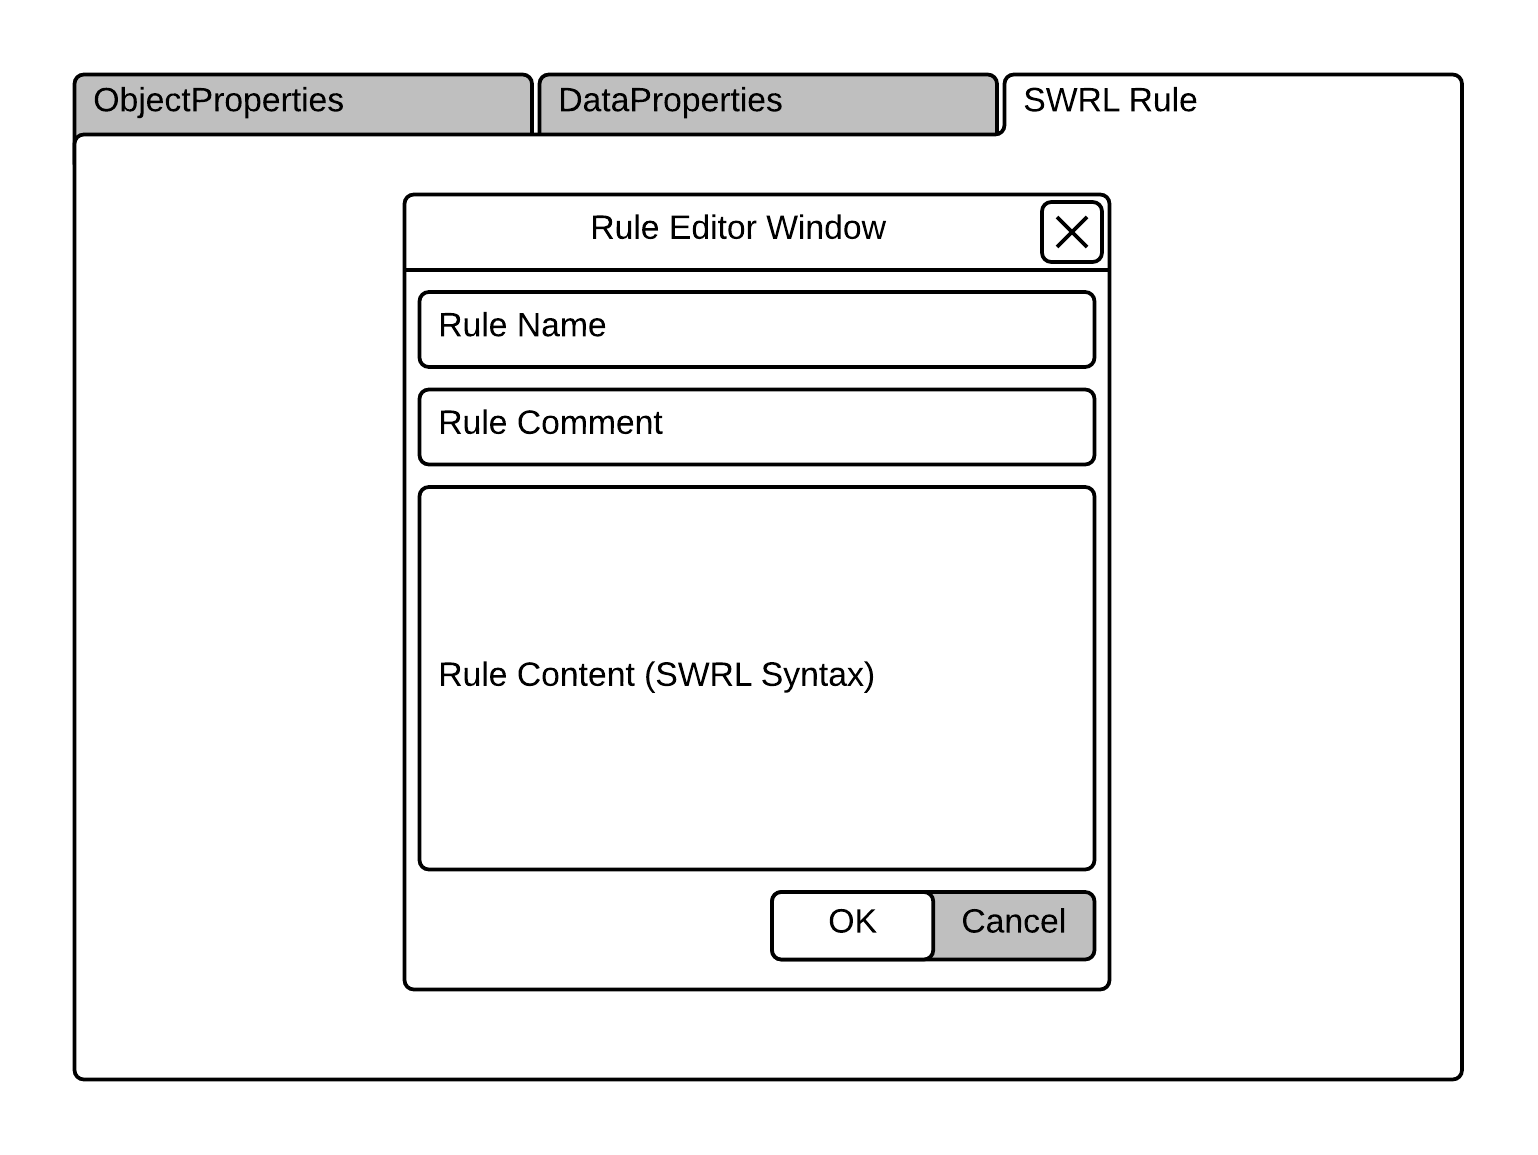
\includegraphics[width=155mm,height=95mm]{Figures/ui_mainview_ruleeditor.png}
	\caption{Phác thảo cửa sổ biên tập rule \label{overflow}}
\end{figure}
Các tab về lớp (Class), thuộc tính đối tượng (Object Propery) và thuộc tính dữ liệu (Data Propery) sẽ có bố cục giống nhau (Hình 3.3). Bên trái là một cây biểu diễn cấu trúc phân cấp của các loại thực thể này và bên phải là các panel nhỏ. Từng panel sẽ tương ứng với từng loại phát biểu có liên quan đến thực thể được chọn bên trái. Riêng tab về các cá thể sẽ có bố cục hơi khác so với các thực thể còn lại, nó sẽ có thêm một danh sách (sẽ nằm bên dưới cấu trúc cây chứa các lớp - Hình 3.4). Bên trong tab SWRL Rules sẽ là một bảng gồm chứa các rule, chia thành 3 cột gồm tên, nội dung và lời chú thích cho rule (Hình 3.5).

Ngoài các view và tab đã kể ở trên, thì ứng dụng buộc phải có thêm các thành phần giao diện hỗ trợ viêc biên tập mô tả lớp, thuộc tính, cá thể (class/property expression, individual assertion axiom) và việc biên tập SWRL Rule. Các hình 3.6, 3.7  thể hiện phác thảo về các giao diện đảm nhiệm những tính năng vừa nêu.
\section{Truy xuất đến các thành phần của Ontology trong OWL-API bằng cách áp dụng Visitor Pattern}
Trong OWL-API, các đối tượng dữ liệu có cấu trúc tương tự với các thành phần trong OWL 2 Ontology (được trình bày trong mục 2.2.3) - tên của các đối tượng dữ liệu sẽ có thêm tiếp đầu ngữ \textit{"OWL"} cộng với tên của thành phần trong OWL 2 như \textit{Ontology} thì đối tượng trong OWL-API sẽ là \textit{OWLOntology}, \textit{ClassExpression} (mô tả lớp) thì đối tượng tương ứng là \textit{OWLClassExpression}, tương tự cho các thành phần khác. Việc tương tác và thay đổi sẽ diễn ra trong đối tượng \textit{OWLOntology} - đối tượng Java biểu diễn một OWL 2 ontology. 
\\
Như đã được giới thiệu trong mục 2.2.3, với một cấu trúc phức tạp gồm nhiều đối tượng được mở rộng và thừa kế từ các loại đối tượng khác, thì việc truy xuất đến từng thành phần cụ thể và áp dụng các thay đổi khác nhau lên chúng là một tác vụ khó nếu không áp dụng Visitor Pattern.
\subsection{Visitor Pattern}
\begin{figure}[h!]
	\centering
	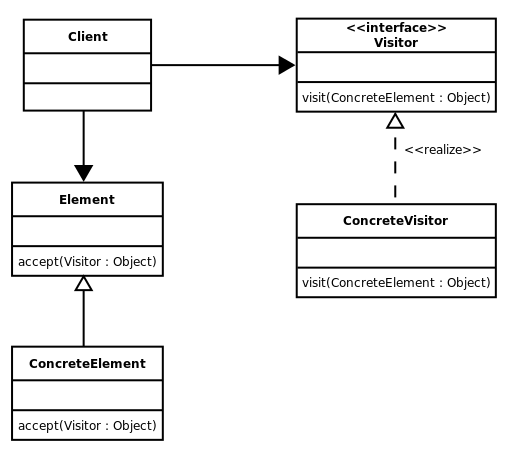
\includegraphics[width=100mm]{Figures/visitor_diagram.png}
	\caption{Visitor Design Pattern\label{overflow}}
\end{figure}
Visitor Pattern là một design pattern trong lập trình hướng đối tượng với mục tiêu tách biệt các cấu trúc dữ liệu khỏi giải thuật. Nói cách khác chúng ta dễ dàng thay đổi các giải thuật mong muốn lên các thành phần của OWLOntology mà không cần phải thay đổi cấu trúc của chúng. Như biểu diễn trong hình mọi loại đối tượng kế thừa/mở rộng từ IElement đều có khả năng truy xuất bởi các đối tượng áp dụng Interface Visitor, các giải thuật mong muốn sẽ được định nghĩa trong phương thức \textit{visit}.
\subsection{Visitor trong OWL-API}
Trong OWL-API cung cấp sẵn một số các Interface Visitor cho từng loại thành phần cụ thể. Ví dụ như OWLClassExpression sẽ có OWLClassExpressionVisitor, hay OWLDatatype sẽ có OWLDatatypeVisitor, .v.v.. . Hình sau đây miêu tả cách hoạt động của OWLClassExpressionVistor.
\begin{figure}[h!]
	\centering
	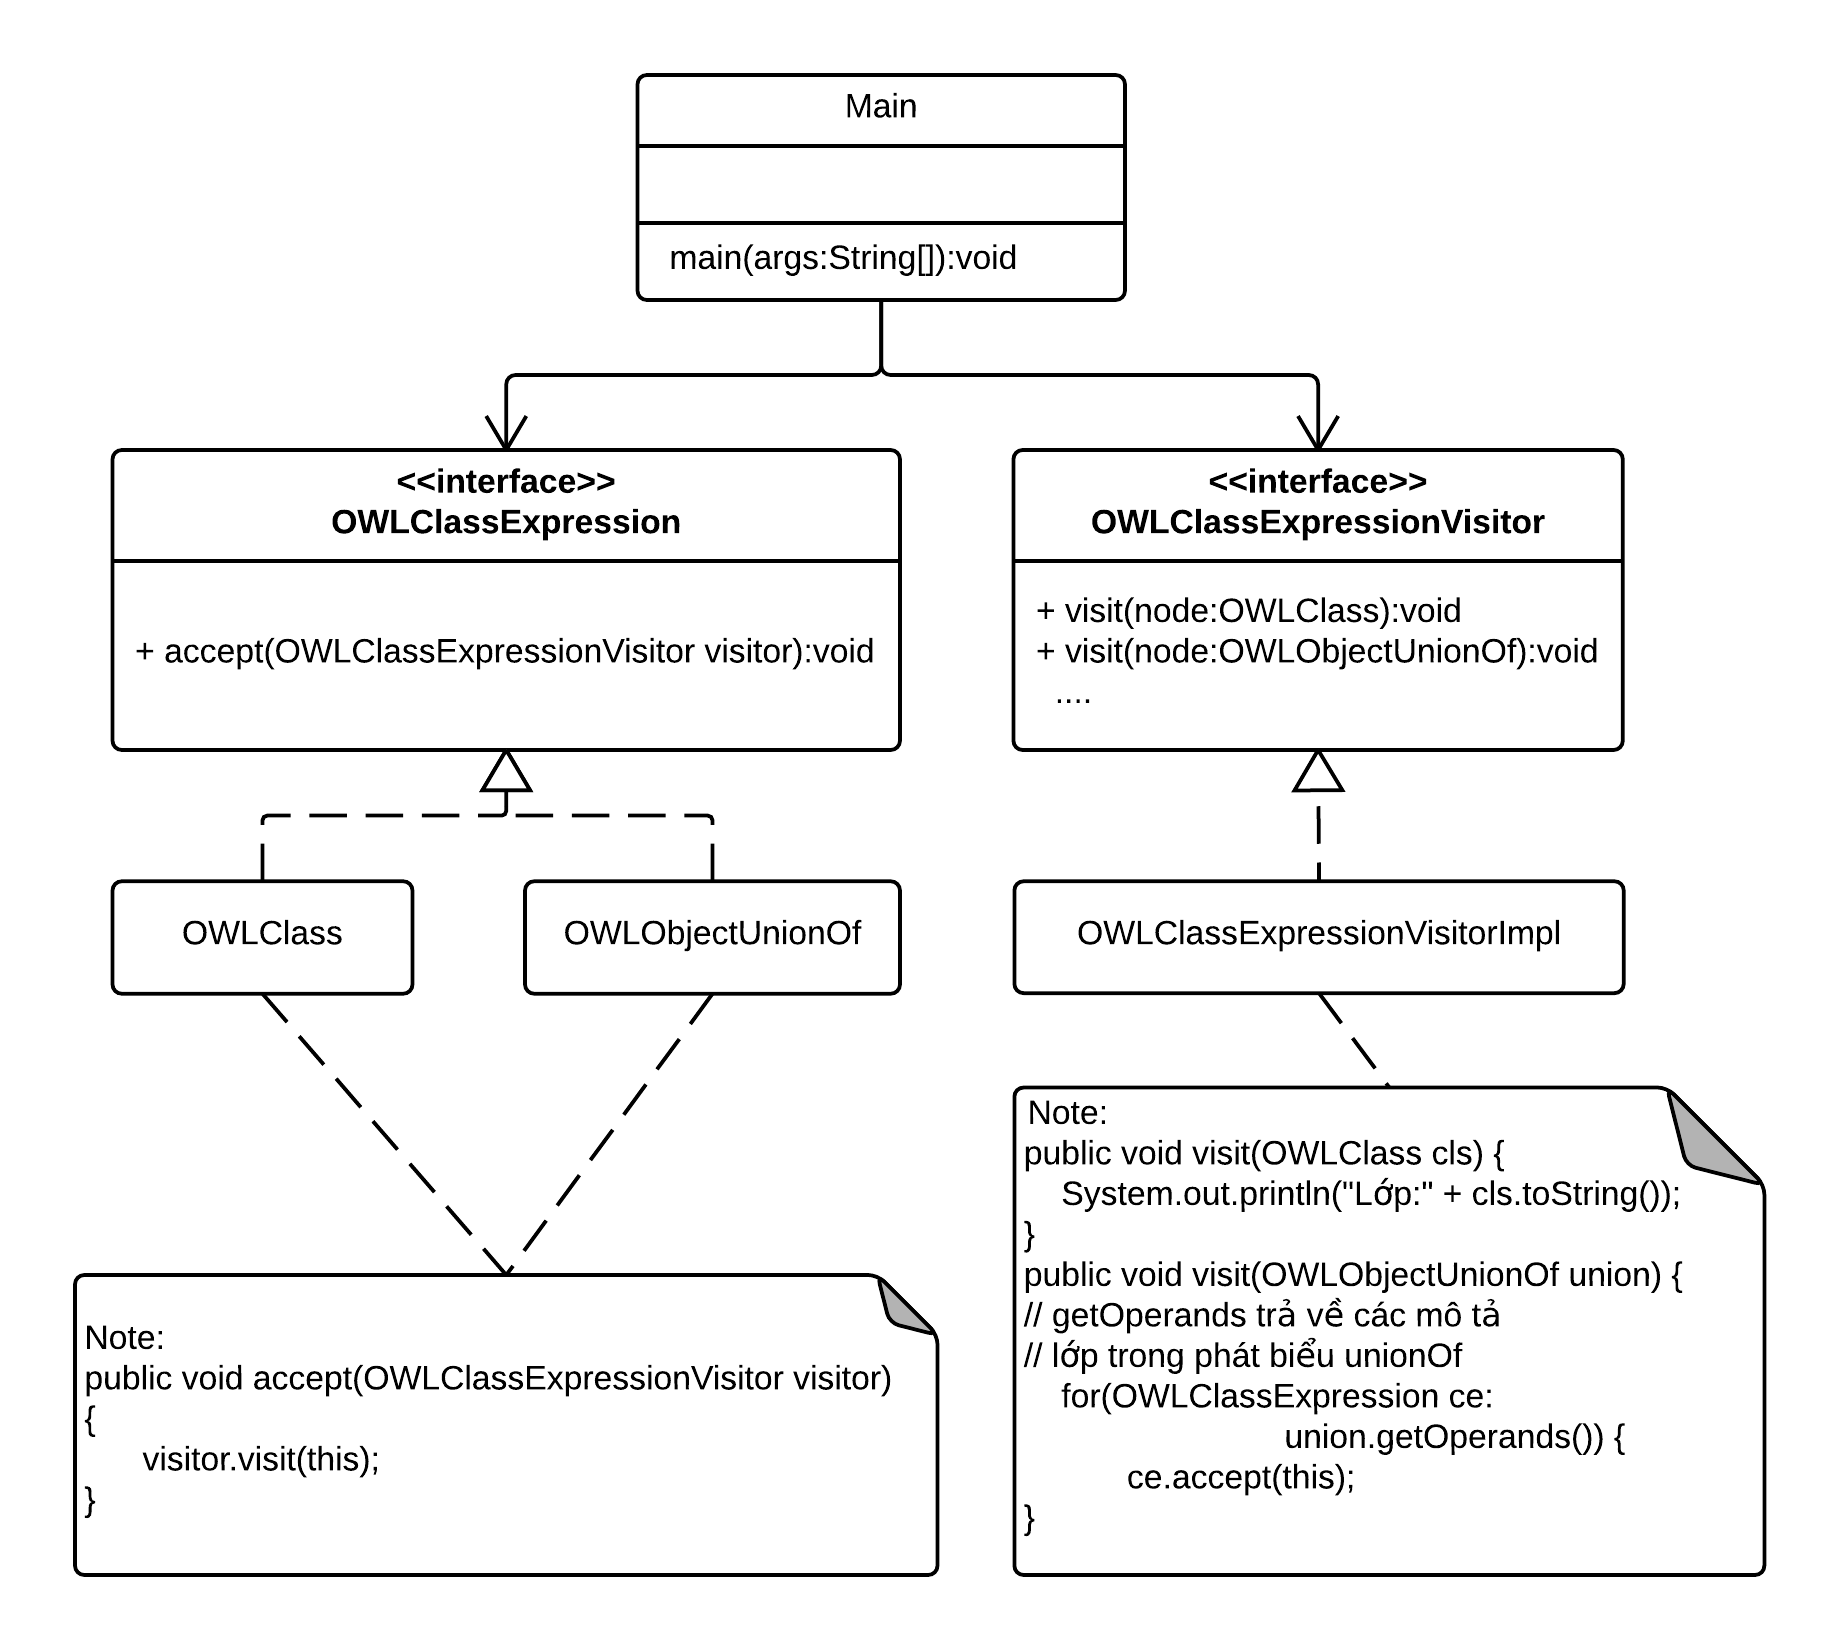
\includegraphics[width=145mm]{Figures/uml_classdiagram_classexpressionvistior_nobackground.png}
	\caption{Class Diagram của OWLClassExpressionVisitor \label{overflow}}
\end{figure}
{\let\thefootnote\relax\footnotetext{*\textit{
		OWLDataFactory: nằm trong OWL-API với chức năng dùng như một nhà máy tạo ra mọi loại đối tượng từ lớp, thuộc tính tới các phát biểu.
}}
Giải sử chúng ta có một mô tả lớp (class expression) bằng Manchester Syntax \textit{"Car and Bike"} và hàm main trong hình khai báo như sau:
\begin{verbatim}
// void main 
OWLDataFactory factory = OWLManager.getOWLDataFactory();
OWLClass car = factory.getOWLClass("a:Car");
OWLClass bike = factory.getOWLClass("a:Bike");
OWLObjectUnionOf union = factory.getOWLObjectUnionOf(car, bike);
OWLClassExpressionVisitor visitor = new OWLClassExpressionVisitorImpl();
union.accept(visitor);
// Ta sẽ có output là 
Lớp: a:Car
Lớp: a:Bike                                       
\end{verbatim}
Visitor lớn nhất trong OWL-API là \textit{OWLObjectVisitor} có khả năng truy vấn đến tất cả các loại đối tượng thuộc \textit{OWLOntology}. Visitor này thực ra được tập hợp lại từ nhiều visitor nhỏ hơn (Hình 3.10).
\begin{figure}[h!]
	\centering
	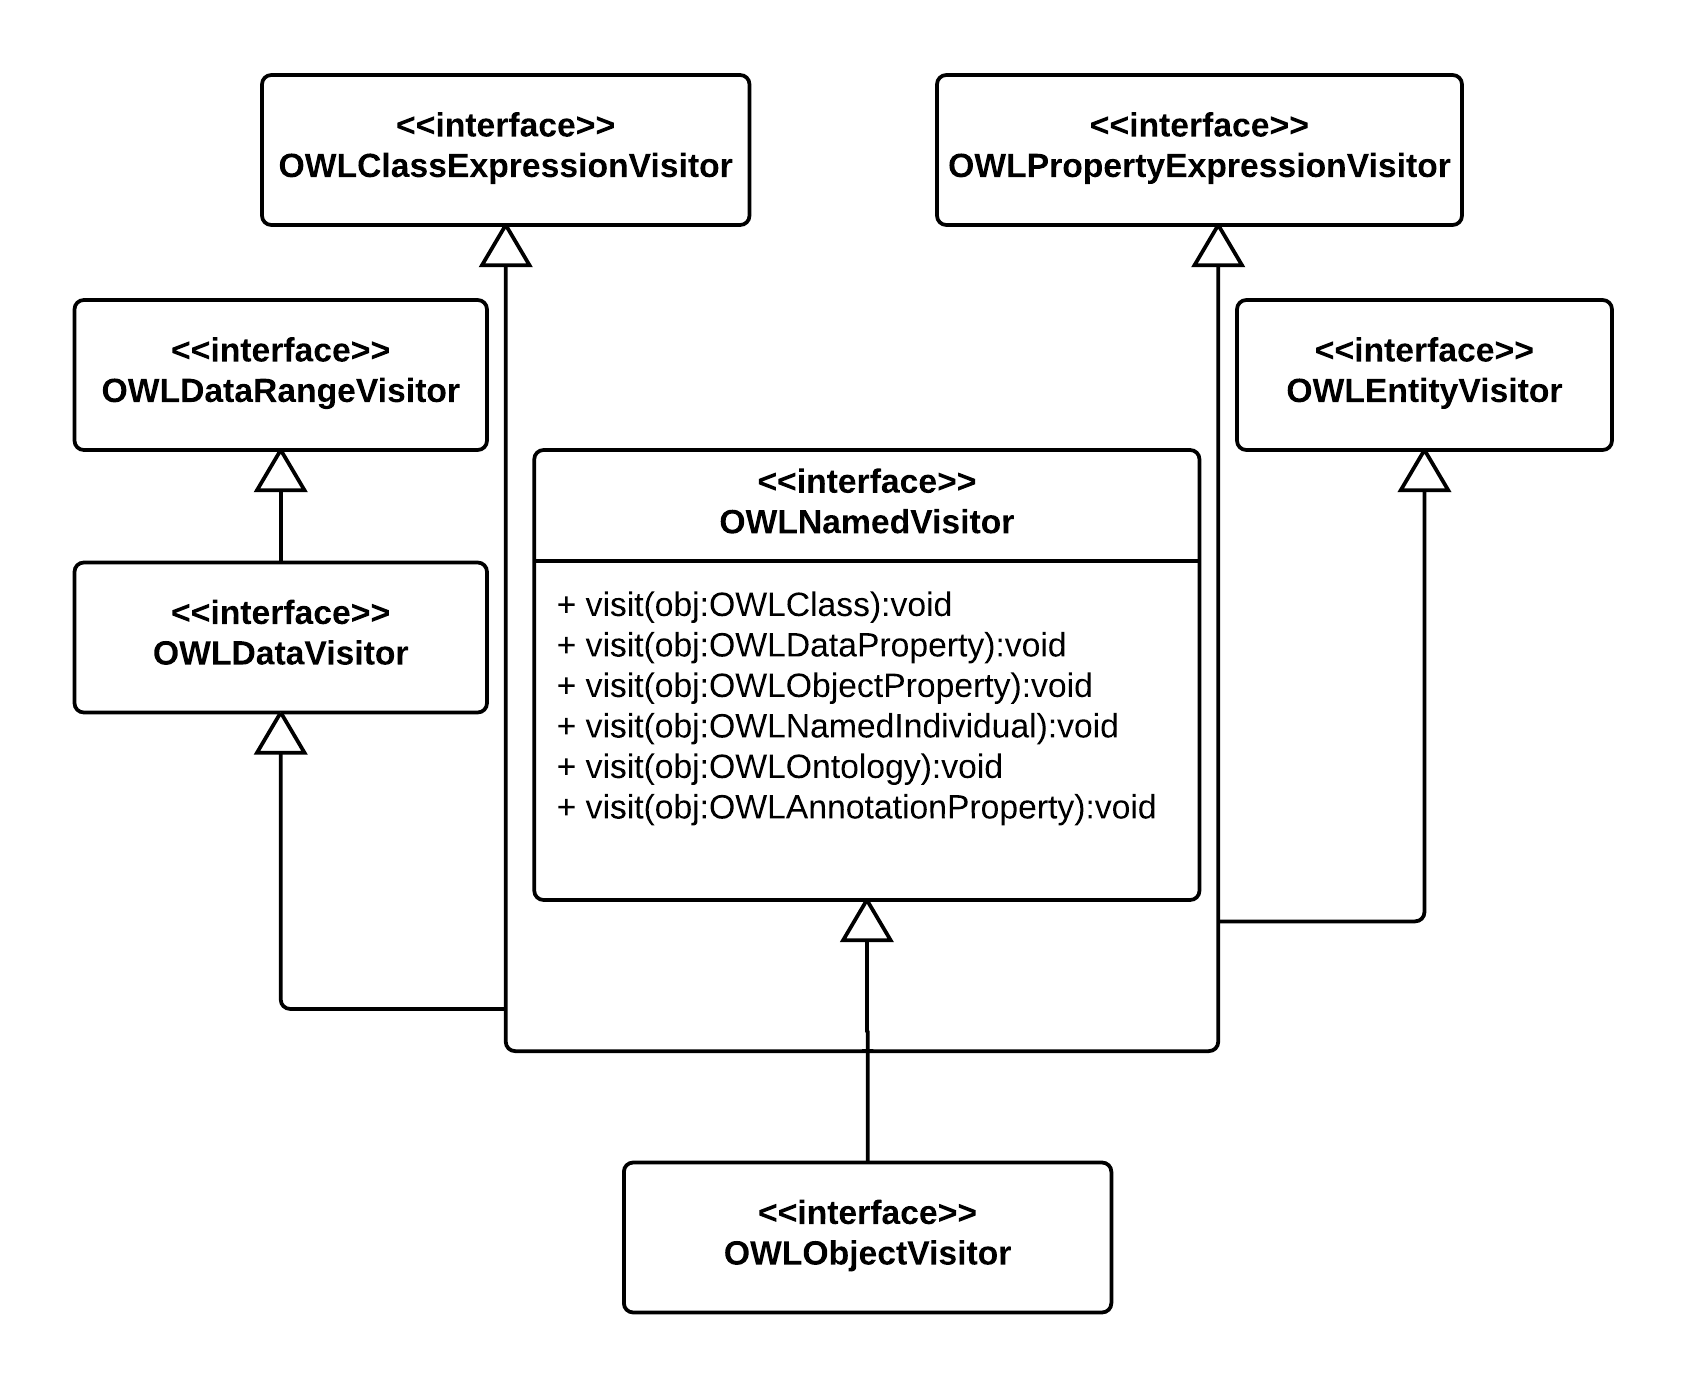
\includegraphics[width=145mm]{Figures/uml_classdiagram_owlobjectvisitor_nobackground.png}
	\caption{Class Diagram của OWLObjectVisitor \label{overflow}}
\end{figure}
Nhờ tận dụng tính đa hình trong lập trình hướng đối tượng nên các loại đối tượng thừa kế/mở rộng từ OWLObject đều có khả năng chấp nhận truy vấn lên chính nó (visitor.visit(this)) từ \textit{OWLObjectVisitor} (Hình 3.11).
\begin{figure}[h!]
	\centering
	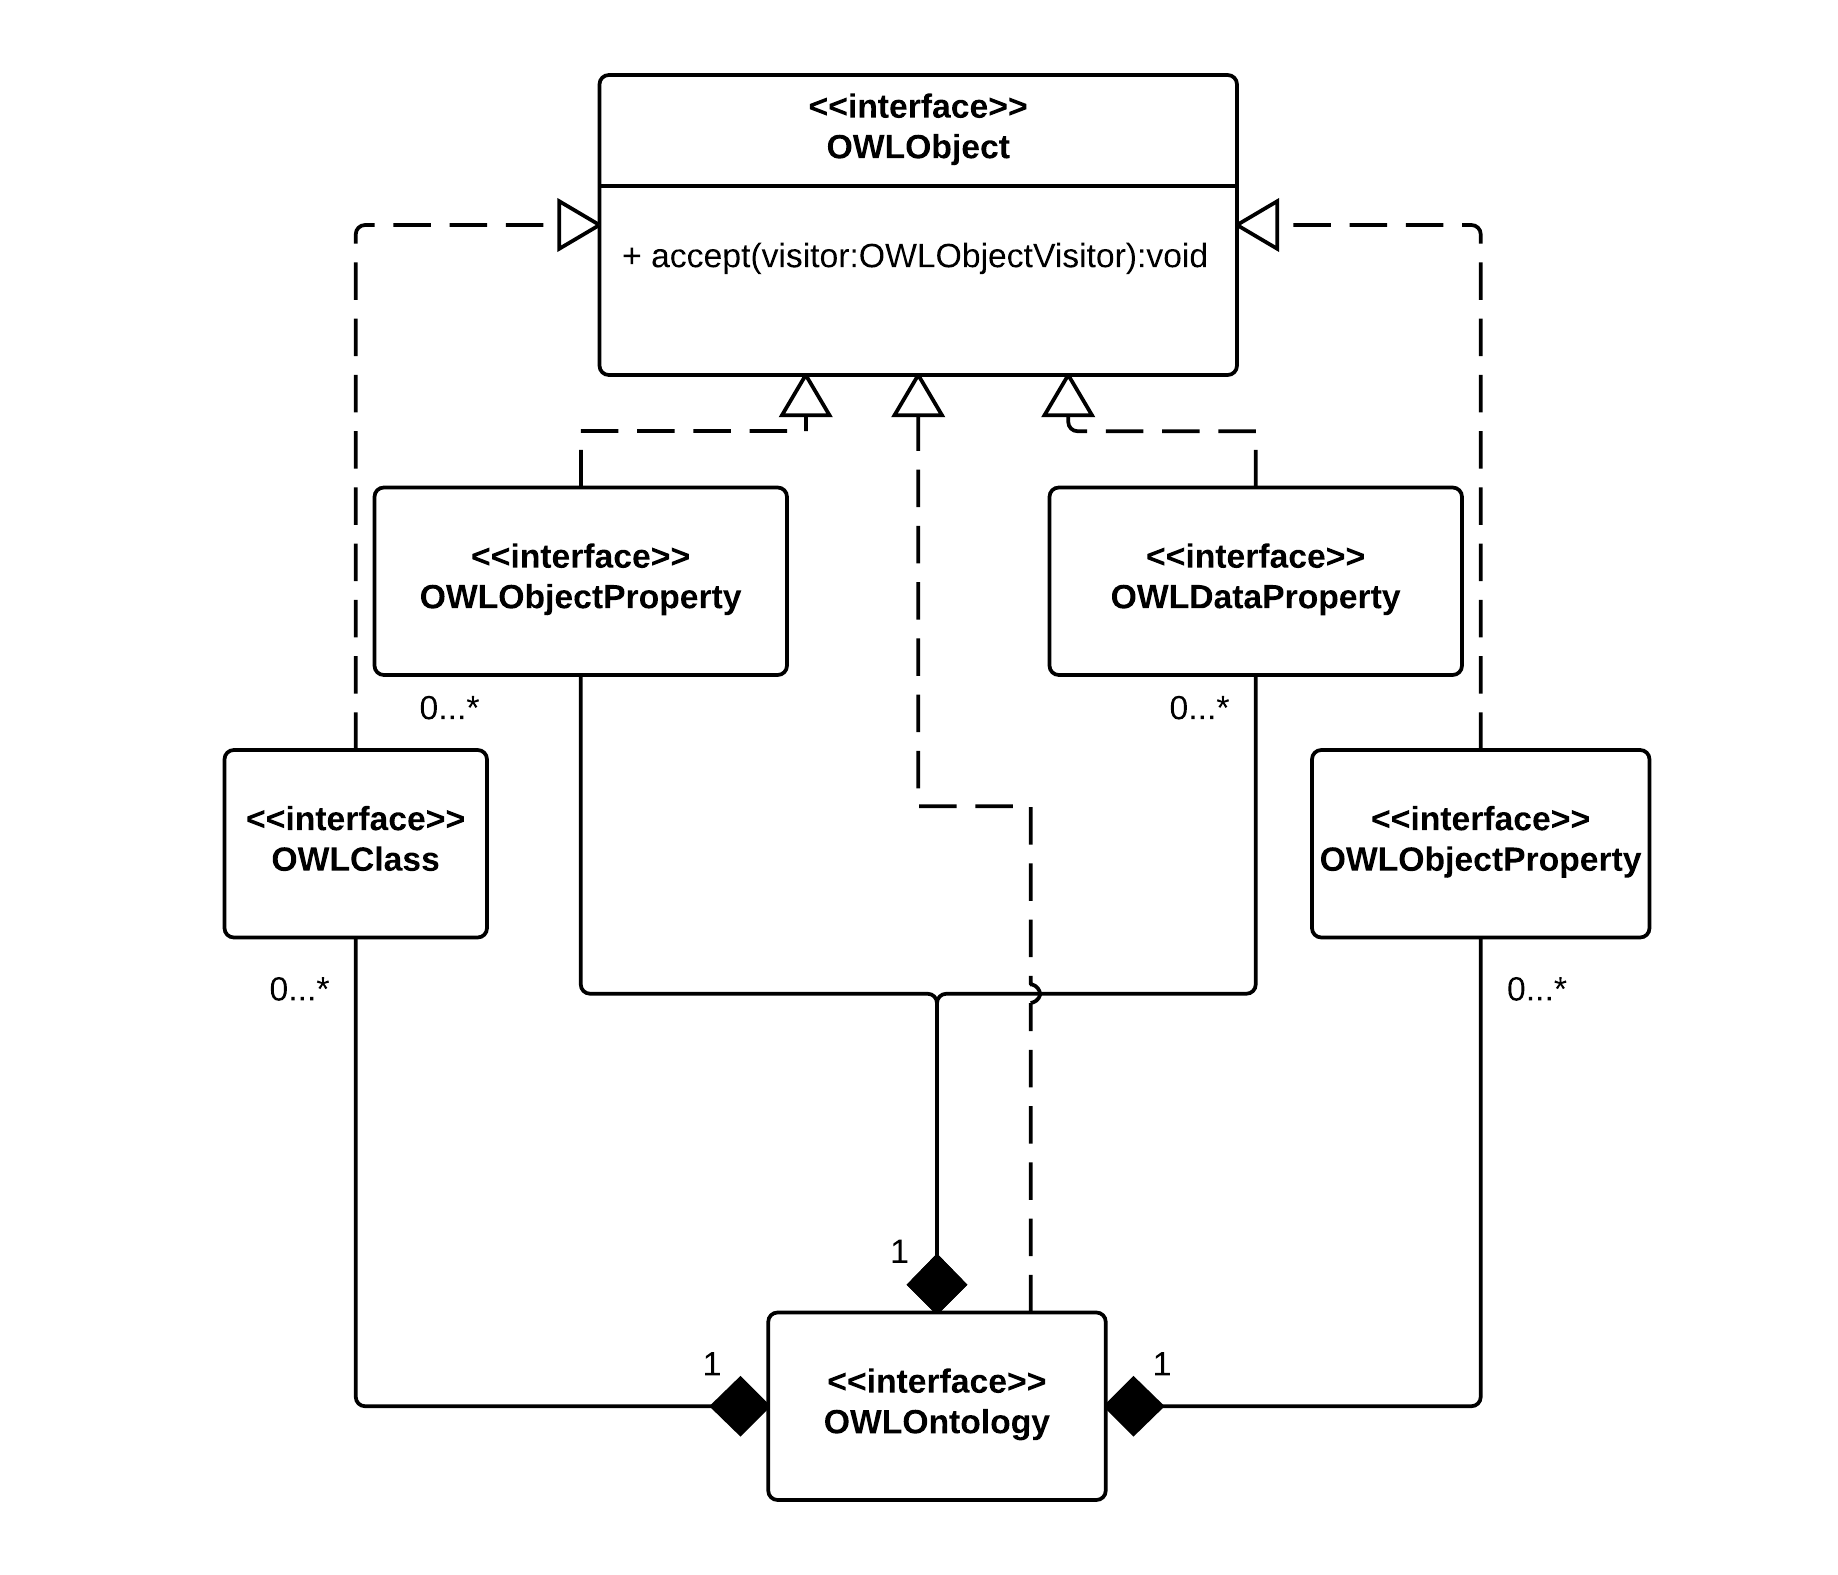
\includegraphics[width=145mm]{Figures/uml_classdiagram_owlobject_forvisitor_nobackground.png}
	\caption{Class Diagram của OWLObject và OWLObjectVisitor \label{overflow}}
\end{figure}
Để sử dụng các visitor, chúng em chỉ cần tạo các class áp dụng các interface tương ứng nhằm truy vấn dạng thành phần cụ thế như ví dụ OWLClassExpressionVisitor ở trên. Tuy nhiên, mỗi lần sử dụng là mỗi lần phải viết lại nội dung các phương thức trong Interface Visitor, để hạn chế sự lặp lại này OWL-API cũng cung cấp sẵn hoặc chúng ta cũng có thể tạo các class VisitorAdapter với nội dung mỗi phương thức được cài đặt tính năng mặc định. Ví dụ:
\begin{verbatim}
ClassExpressionVisitorAdapter implements OWLClassExpressionVistor {
  private void doNothing(OWLClassExpression ce) {};
  public void visit(OWLClass cls) {doNothing(cls);}
  public void visit(OWLObjectUnionOf union) {doNothing(cls);} ... }
\end{verbatim}
Mỗi khi muốn thay đổi nội dung phương thức nào chỉ cần \textit{Override} lại phương thức đó trong VisitorAdapter là được.
\section{Các tổ chức dữ liệu (data model) cho hệ thống}
Trong Vaadin Framework, dữ liệu trong lúc một ứng dụng đang ở trong tiến trình hoạt động được tổ chức thành các mô hình gọi là Data Model, với 3 cấp khác nhau gồm:Property, Item và Container. Có thể xem các \textit{Data Model} này như một đối tượng bao bọc (encapsulation) lại dữ liệu kiểu dữ liệu mà chúng ta muốn định nghĩa. Nếu câu hỏi là tại sao phải tốn công đưa các dữ liệu vào trong các đối tượng chứa như vậy, thì câu trả lời là vì Vaadin Framework cung cấp một cơ chế mà khi chúng ta tương tác với dữ liệu trong các \textit{Data Model} này thì đồng thời những thành phần giao diện (UI Components) cũng sẽ cập nhật các thay đổi đó. Lý do là vì hầu hết các thành phần giao diện đều được thiết kế độc lập với dữ liệu, dữ liệu được liên kết với các giao diện thông qua các \textit{Data Model} này. Sau đây chúng em xin trình bày cách tổ chức các đối tượng từ OWL-API vào trong các \textit{Data Model} là Property và Container (Item không được sử dụng vì không phù hợp với cấu trúc dữ liệu mà chúng em muốn tổ chức).

\subsection{Tổ chức các đối tượng OWL-API vào trong Property của Vaadin}
\begin{figure}[h!]
 	\centering
 	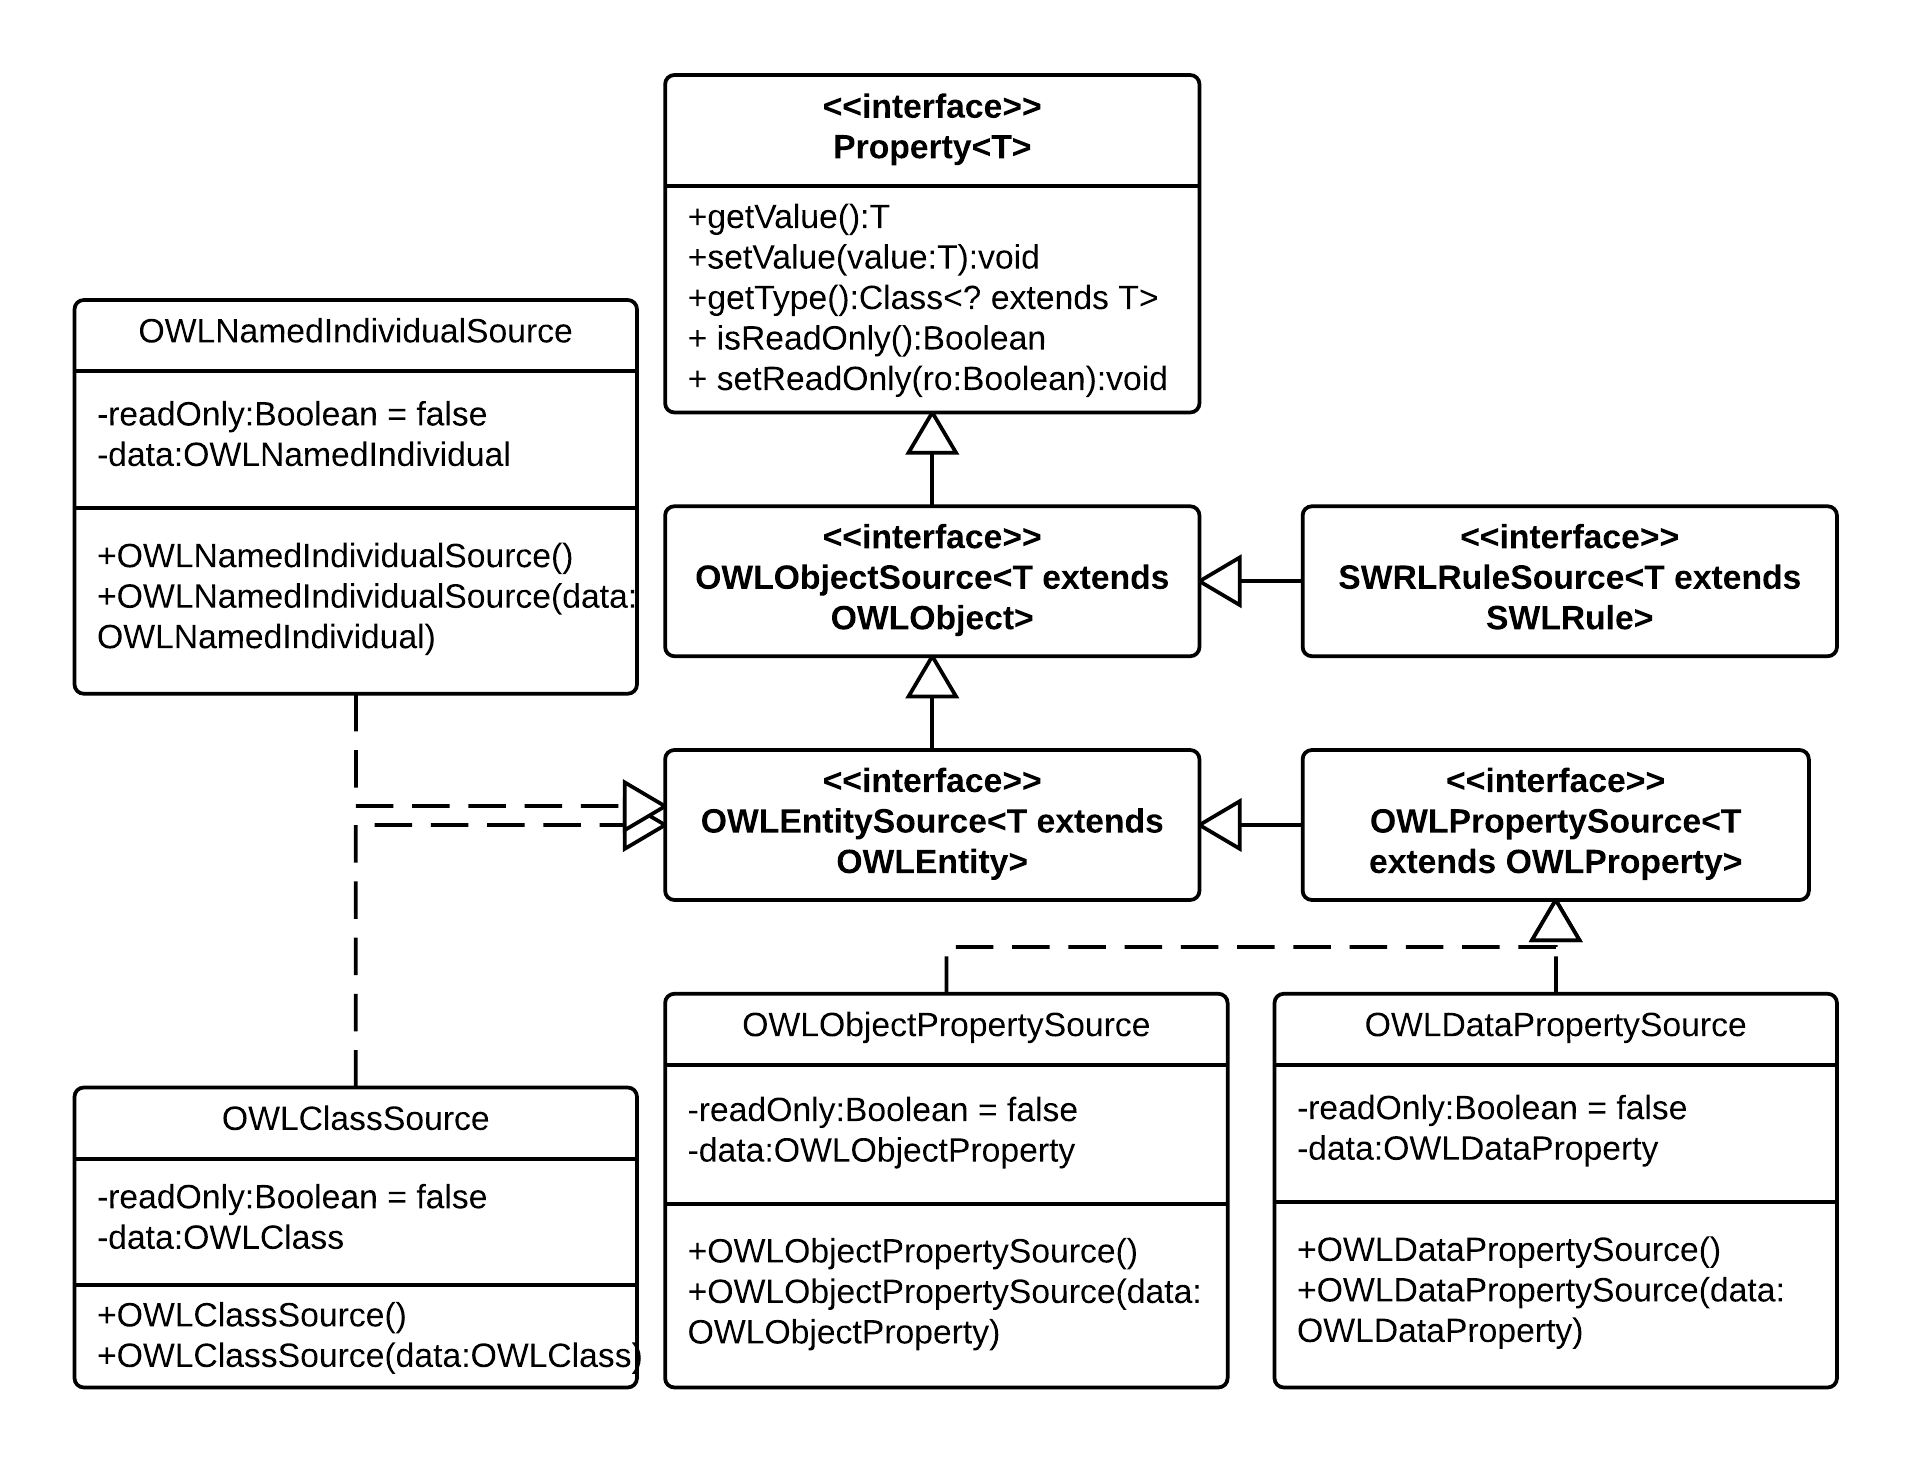
\includegraphics[width=150mm]{Figures/uml_owleditor_owlobjectsource.png}
 	\caption{Class Diagram của Property<T>\label{overflow}}
\end{figure}
\textbf{Property} là \textit{Data Model} đơn giản nhất, được Vaadin cung cấp dưới dạng Interface \textit{Property<T>} với $T$ kiểu dữ liệu được chúng ta định nghĩa, các thành phần giao diện như \textit{TextField}, \textit{Label}, \textit{TextArea} sử dụng \textit{Property} để liên kết dữ liệu với các đối tượng dữ liệu được định nghĩa qua $T$. Công việc phải làm là định nghĩa các \textit{Property} chứa các đối tượng OWL-API này. Do tính chất của OWL 2, ta có thế nói OWLClass (lớp) là một OWLEntity (thực thể), OWLEntity là một OWLObject (thành phần của OWL 2). Theo đó mà chúng em cũng sẽ tạo ra các Property tương ứng OWLObjectSource > OWLEntitySource > OWLClassSource. Việc tận dụng tính đa hình của đối tượng rất có ích khi xây dựng các UI Component chung cho các loại đối tượng giống nhau như OWLClass, OWLObjectProprerty, OWLDataProperty (cả đều mở rộng từ OWLEntity). 
\subsection{Tổ chức các thực thể OWLClass, OWLObjectProperty và OWLDataProperty thành các Container}
\begin{figure}[h!]
	\centering
	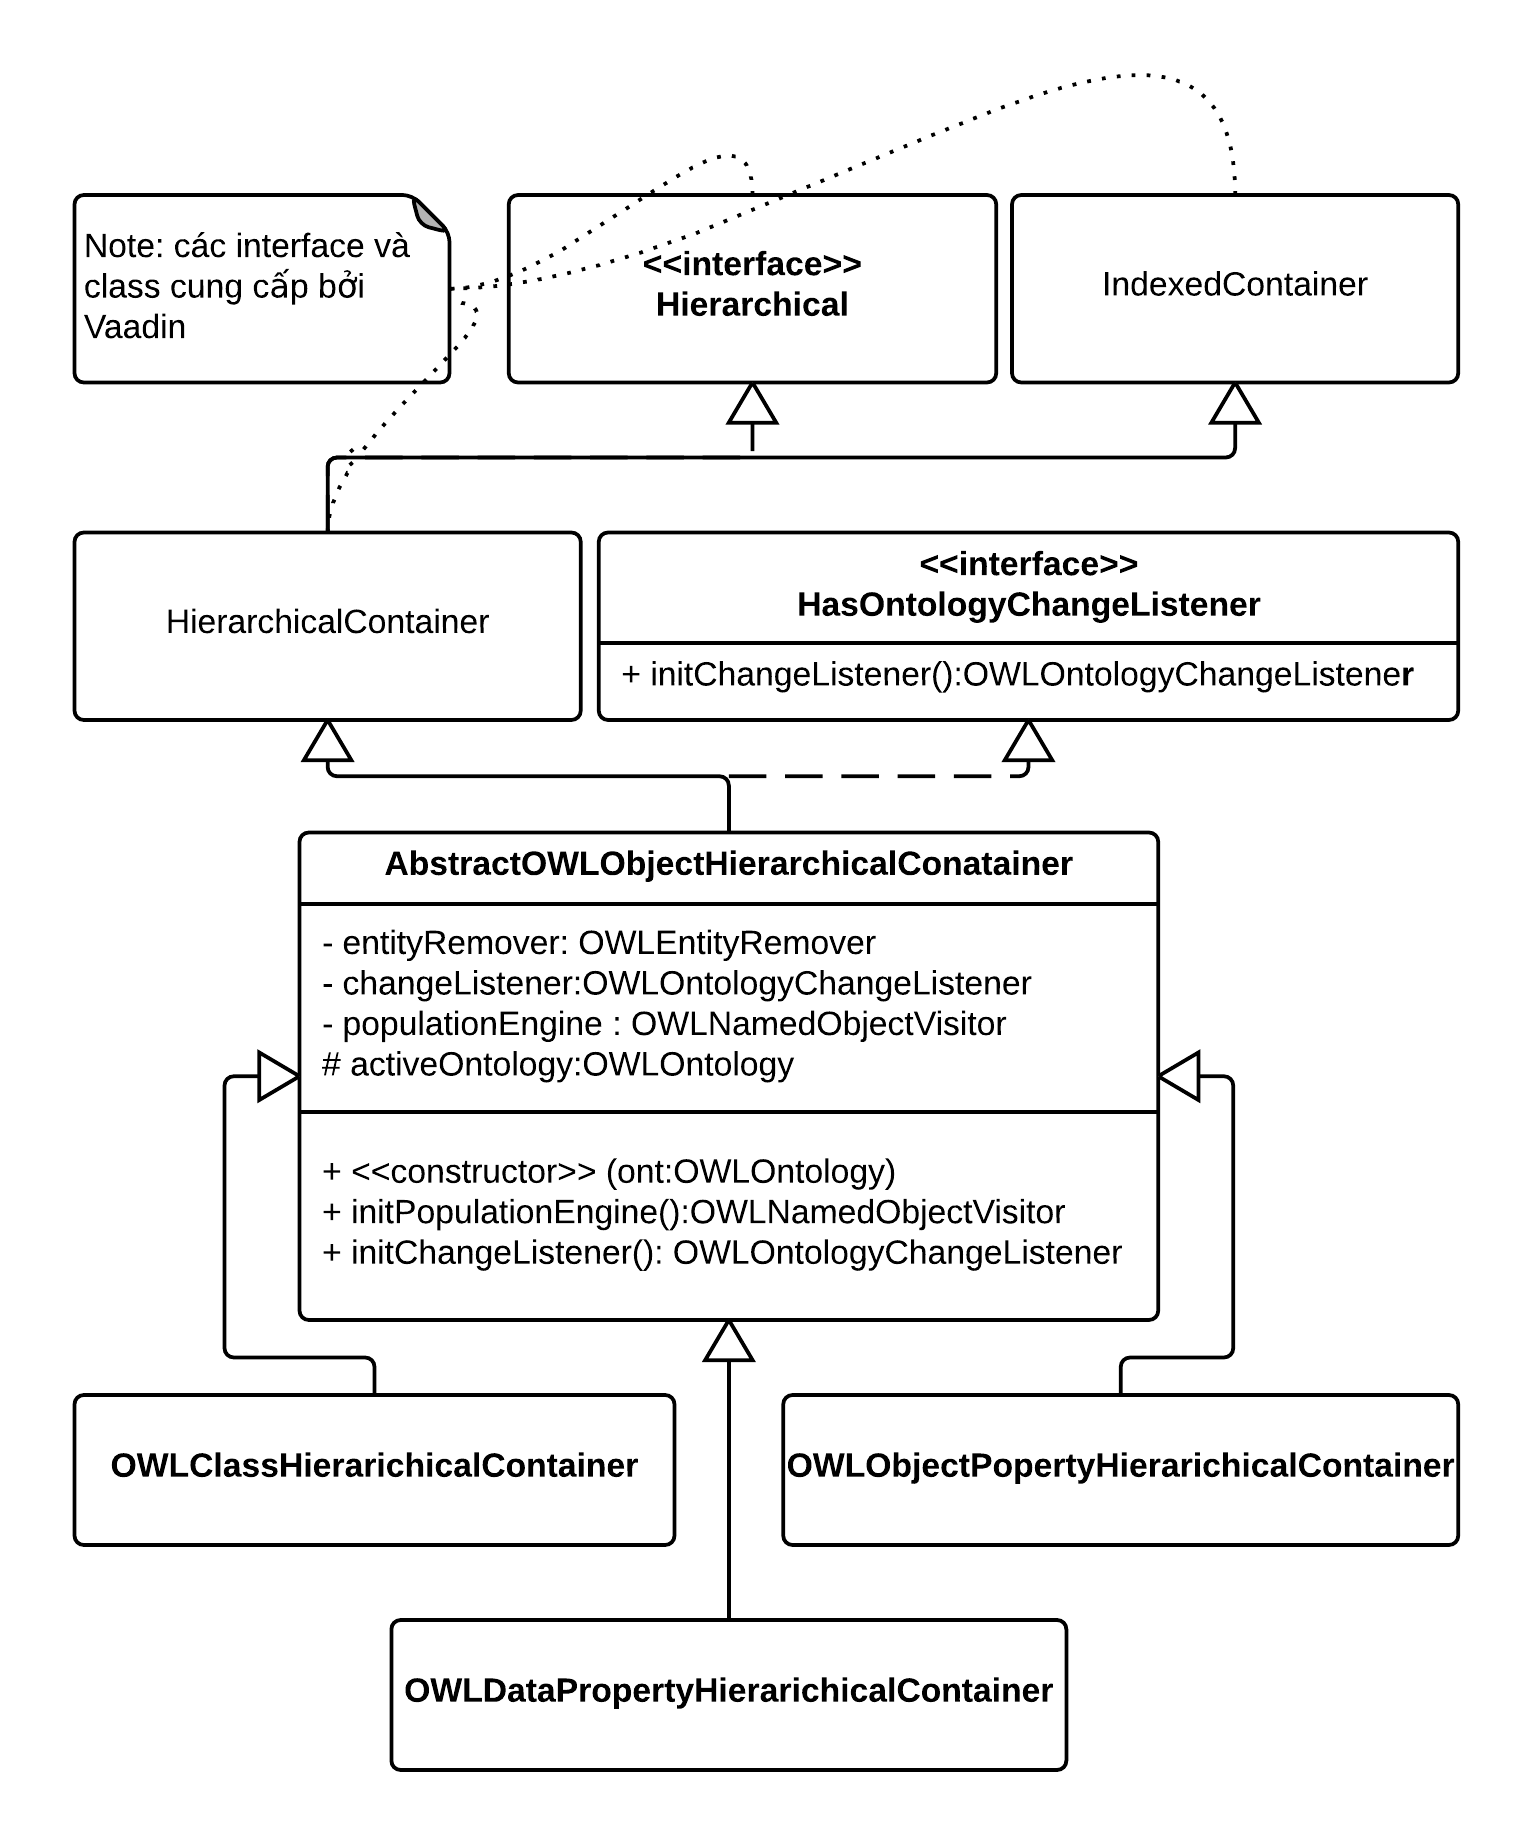
\includegraphics[width=150mm]{Figures/uml_owleditor_abstractcontainer_nobackground.png}
	\caption{Class Diagram của HierarchicalContainer \label{overflow}}
\end{figure}
\textbf{Container} là cấu trúc \textit{Data Model} phức tạp và cao nhất, chúng được chia thành các loại khác nhau tương ứng với tính chất của cấu trúc dữ liệu như \textit{HierarchicalContainer} dùng cho các cấu trúc dữ liệu phân cấp được hỗ trợ trong các thành phần giao diện (UI Component) như \textit{Table}, \textit{Tree}, \textit{ComboBox} và \textit{ListSelect}, đơn giản hơn có \textit{IndexedContainer} dùng cho cấu trúc dữ liệu dạng danh sách được hỗ trợ bởi \textit{ComboBox} và \textit{ListSelect} và \textit{JPAContainer} dùng cho các dữ liệu dạng SQL Table - hỗ trợ bở \textit{Table}, \textit{TreeTable}. Trong ứng dụng, chúng em chỉ sử dụng \textit{HierarchicalContainer} để tổ chức các lớp, thuộc tính đối tượng hay dữ liệu vì chúng cũng có tính chất phân cấp (SubClassOf, SubPropertyOf). Ở đây chúng em cũng xây dựng một AbstractClass rồi mở rộng ra với từng loại OWLEntity tương ứng là OWLClass, OWLObjectProperty và OWLDataProperty (Hình 3.13).

\section{Thiết kế cách xử lý sự kiện}
\subsection{Sử dụng Guava EventBus}
Do hệ thống gồm nhiều tab và các cửa sổ nhỏ (mô tả trong mục phác thảo giao diện), nên chúng em sẽ không áp dụng cách xử lý sự kiện truyền thống trong Java cho toàn hệ thống. Thay vào đó chúng em sử dụng một giải pháp thay thế là thư viện Guava EventBus - một nhánh nhỏ của thư viện Guava phát triển bởi Google \cite{guava}. Với Guava EventBus, mọi thành phần giao diện sẽ đăng ký các phương thức Subscriber - mỗi subscriber sẽ xử lý cho một loại sự kiện cụ thể -  với EventBus trong lúc khởi tạo hoặc hậu khởi tạo, sau đó EventBus lắng nghe mọi sự kiện được công bố lên eventBus bằng phương thức \textit{post}, cuối cùng EventBus bắt sự kiện và truyền sự kiện này đến đúng cho Subscriber nào đã đăng ký xử lý loại sự kiện này lúc đầu (Hình 3.14).
\begin{figure}[h!]
	\centering
	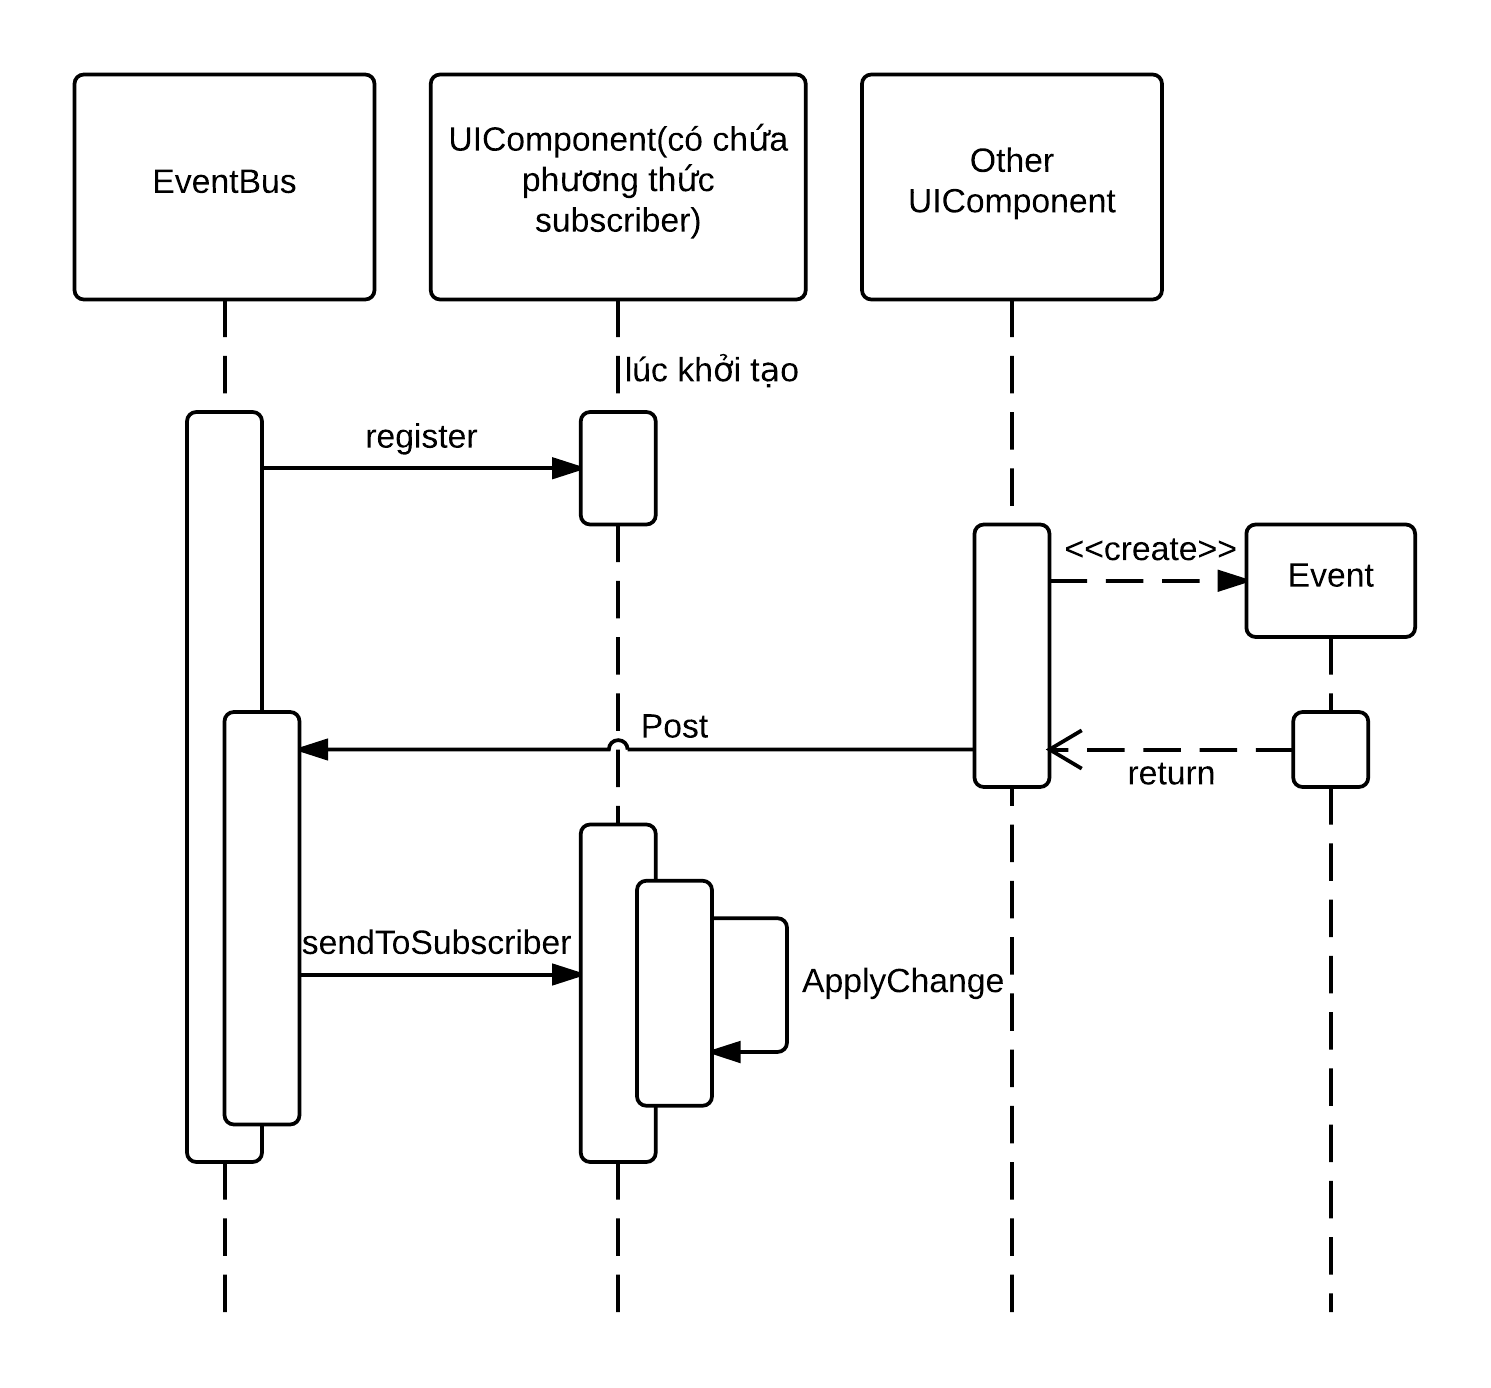
\includegraphics[height=115mm]{Figures/uml_eventbus_sequence.png}
	\caption{Sequence Diagram của EventBus \label{overflow}}
\end{figure}
\\
UIComponent có thể được khai báo subscriber bằng Annotation @Subscribe cung cấp bởi thư viện Guava như sau:
\begin{verbatim}
public class SubscriberComponent {
  public SubscriberComponent { EventBus.register(this); }
  @Subscribe public void eventHandler(SpecificEventType event) { 
  	// các thay đổi được áp dụng ở đây  }
}
\end{verbatim}
EventBus có thể được sử dụng qua một lớp static với các phương thức register, post, unregister. Phương thức được chọn làm subscriber phải đáp ứng các yêu cầu sau đây:
\begin{itemize}
\item Khai báo public
\item Có duy nhất một tham số là sự kiện (event).
\item Không có kiểu trả về (return void).
\end{itemize}
\subsection{Các loại sự kiện trong hệ thống}
Do EventBus sẽ dựa vào loại Event để truyền đến đúng Subscriber cụ thể. Vì thế các loại sự kiện trong hệ thống sẽ được chúng em phân thành 3 loại dạng là thêm (add/create), xóa(remove), sửa (edit/modify) và phân thành 2 loại lớn là các sự kiện liên quan tới các thực thể và các sự kiện liên quan đến các phát biểu.
\begin{figure}[h!]
	\centering
	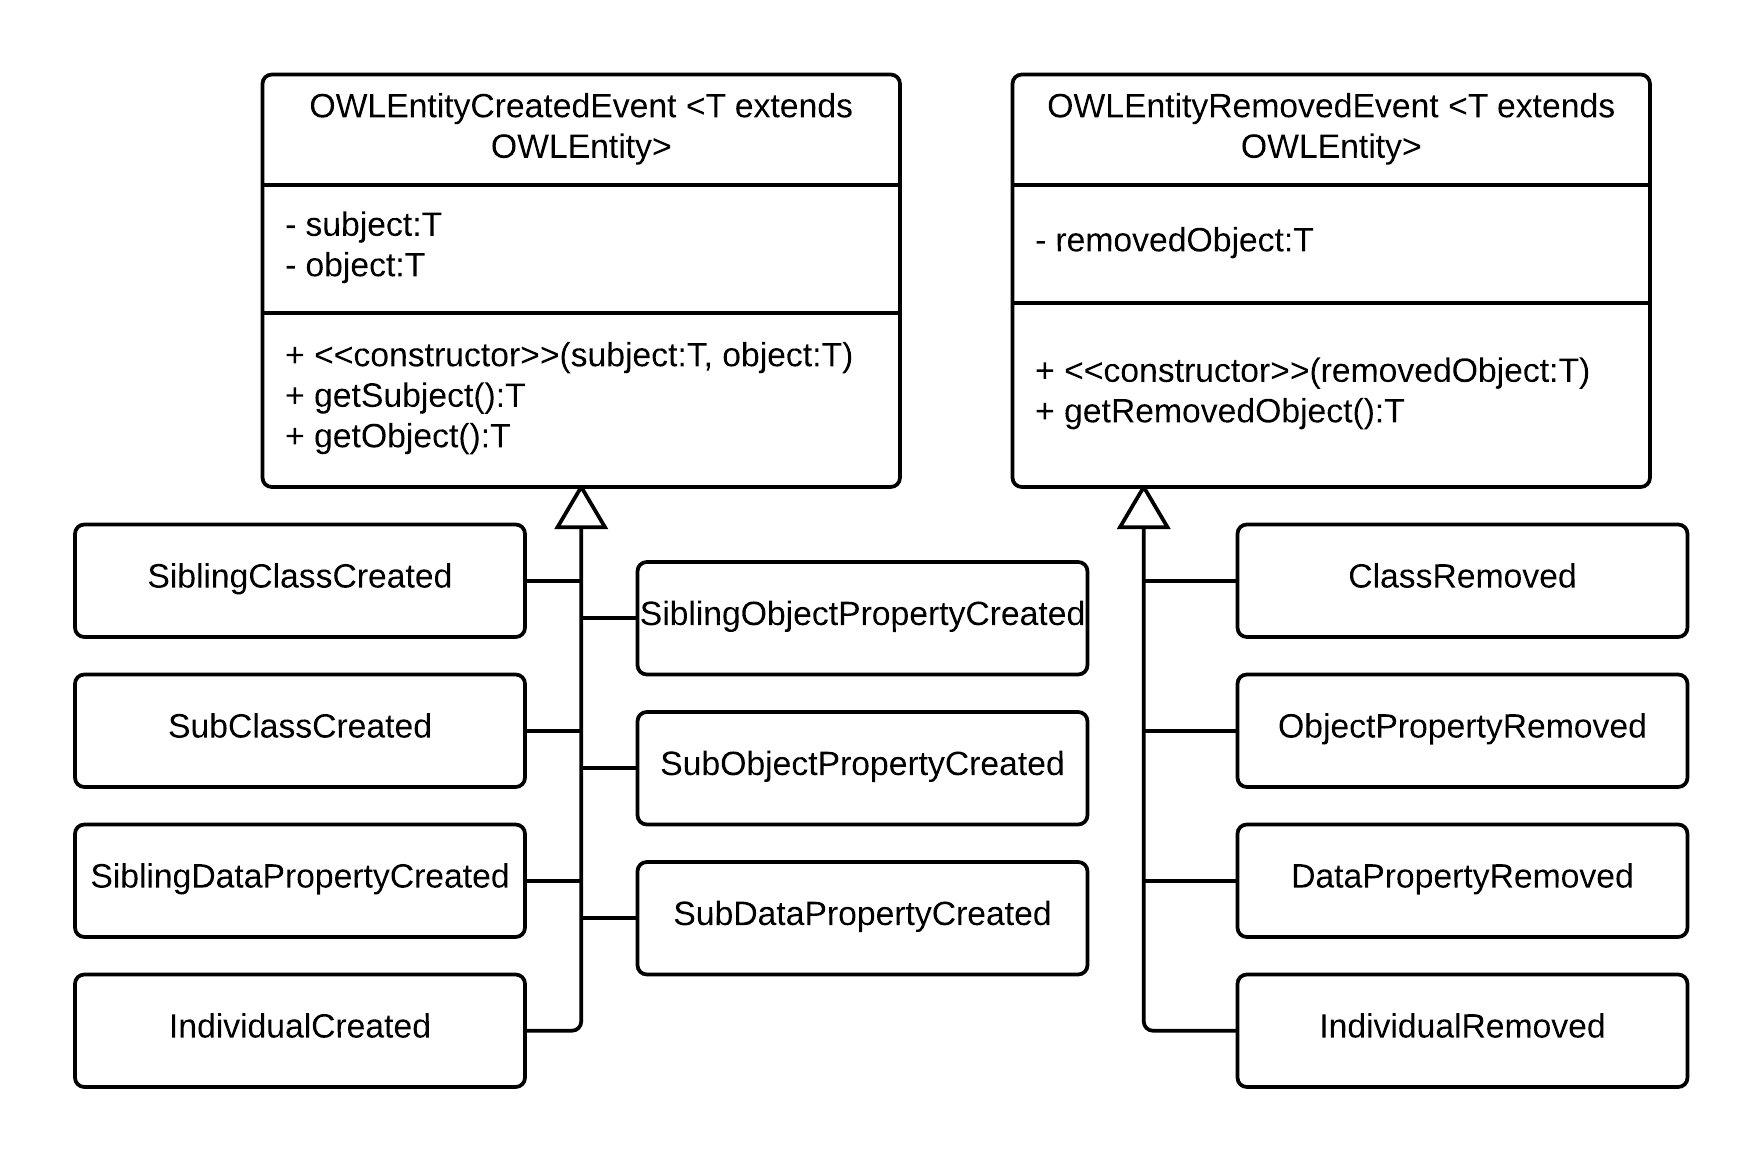
\includegraphics[width=150mm]{Figures/uml_entity_event.png}
	\caption{Class Diagram của các sự kiện liên quan đến thực thể\label{overflow}}
\end{figure}
\begin{figure}[h!]
	\centering
	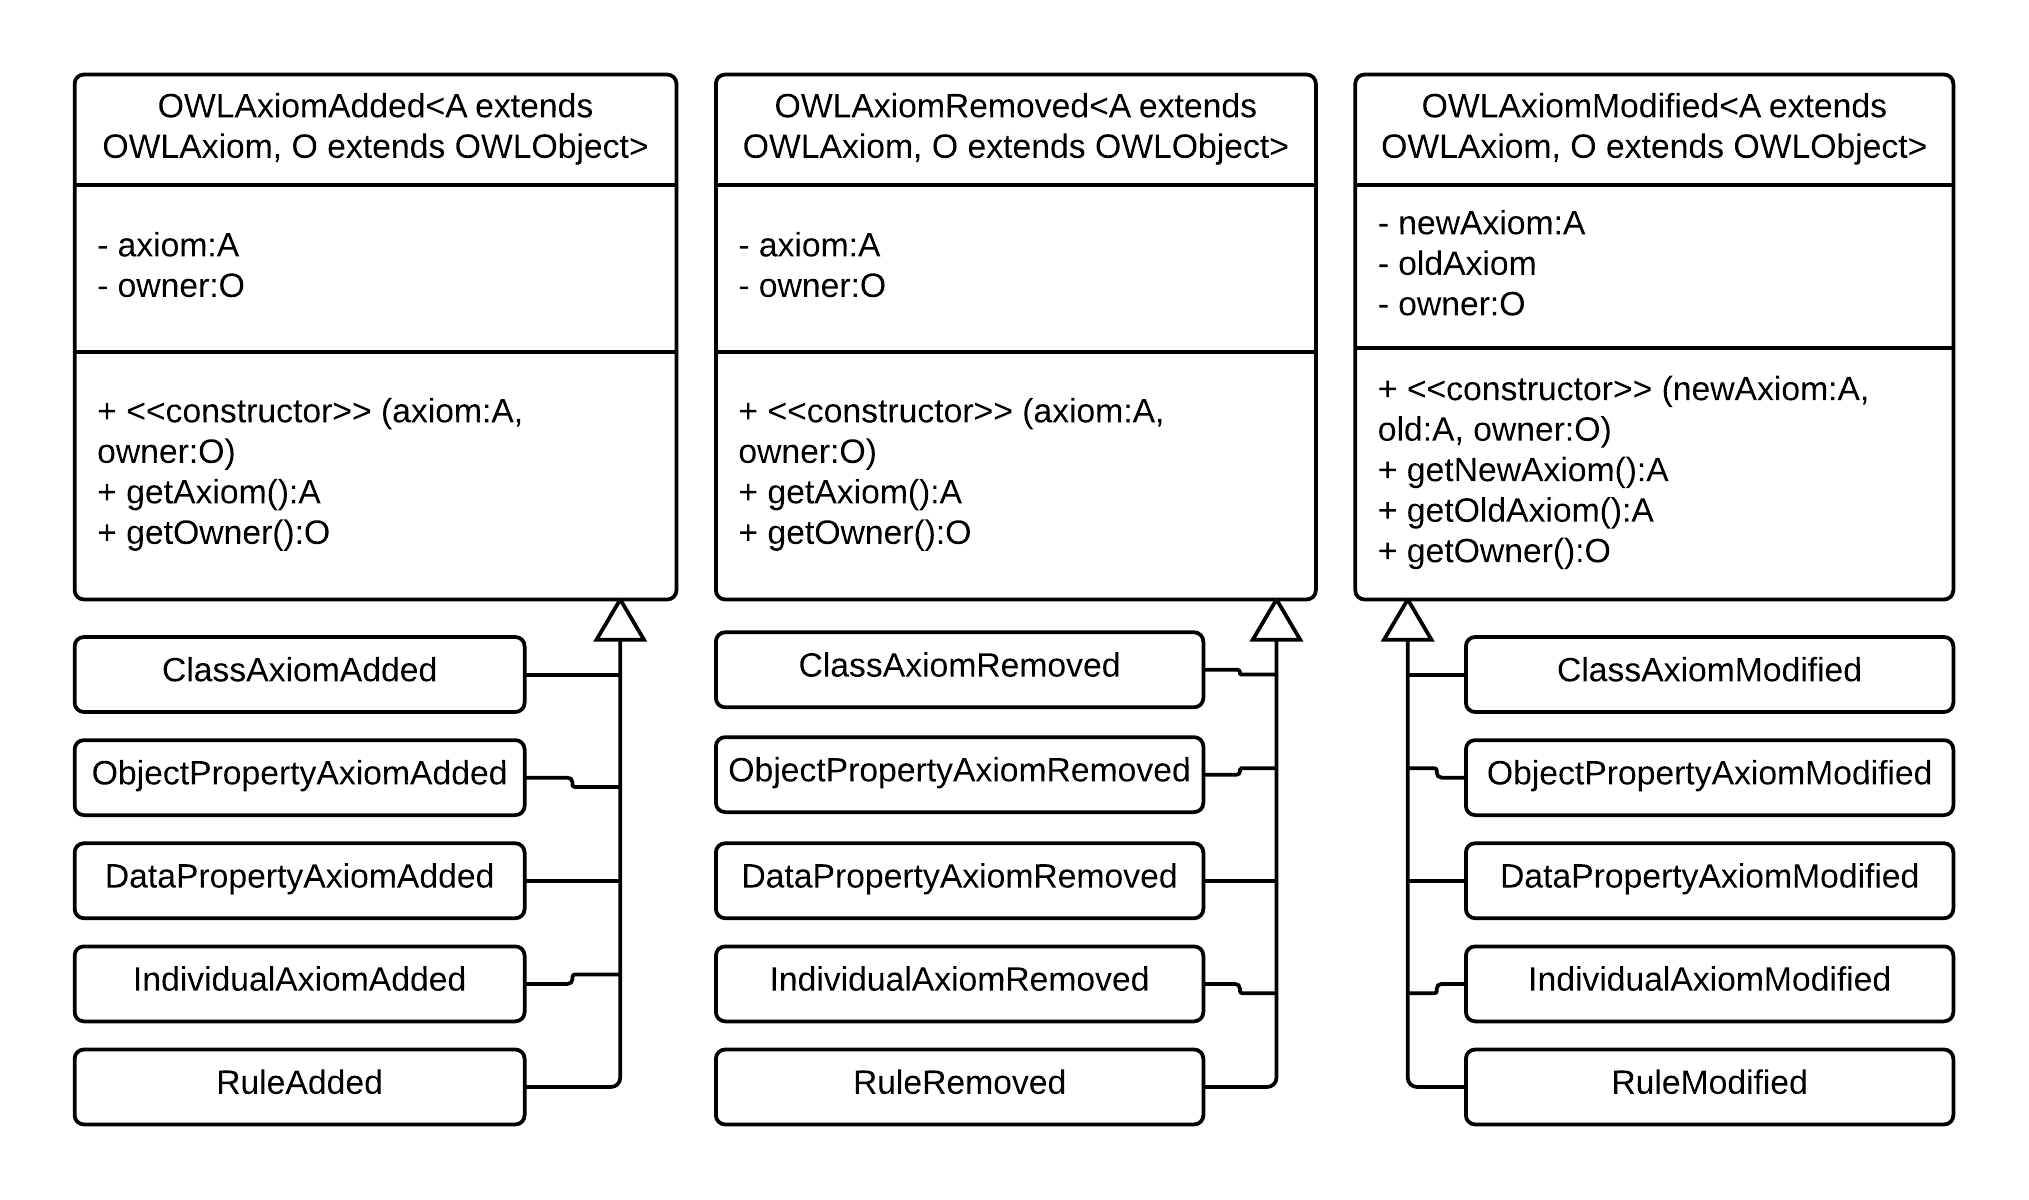
\includegraphics[height=97mm]{Figures/uml_axiom_event.png}
	\caption{Class Diagram của các sự kiện liên quan đến các phát biểu \label{overflow}}
\end{figure}
Tên của các sự kiện cho cá thể gồm phần đầu là tên loại thực thể (Class, ObjectProperty, ...) và phần sau là động từ nói lên đó là sự kiện thêm, xóa hay sửa (Hình 3.15). Đối với sự kiện dành cho các phát biểu, tên của chúng gồm phần đầu nói lên loại phát biểu mà sự kiện đó đang xử lý và phần sau là động từ nói lên hành động thêm, xóa hay sửa (Hình 3.16).
\\
\section{OWLEditorKit}
\begin{description}
	\item[Interface:] \verb|vn.edu.uit.owleditor.OWLEditorKit|
	\item[Class implementation:] \verb|vn.edu.uit.owleditor.OWLEditorKitImpl|
\end{description}
Đây là thành quan trọng nhất của toàn bộ hệ thống được thiết kế để đảm nhiệm việc khai thác các API từ OWL-API, nạp/tạo Ontology từ IRI, suy luận, giải thích các phát biểu, parse các chuỗi viết theo cú pháp \textit{Manchester} thành các mô tả lớp và dữ liệu. Thực ra, các chứng năng vừa kể trên hầu hết đều được thực thi nhờ các API của OWL-API, \textit{OWLEditorKit} đóng gói tất cả lại thành một đối tượng để dễ dàng sử dụng trong các UI Component hơn, cũng như tránh việc phải khởi tạo nhiều lần các API. 
\subsection{Các chức năng của OWLEditorKit}

\subsubsection{Nạp Ontology}
Tương ứng với hàm \textit{loadOntologyFromOntologyDocument}, load các tài liệu OWL2 từ tham số là đối tượng \textit{IRI} của OWL-API, ontology khi load xong sẽ được gán cho đối tượng Active Ontology (sẽ được đề cập ngay sau).
\begin{verbatim}
OWLEditor kit = new OWLEditorKitImpl();
kit.loadOntologyFromOntologyDocument(IRI.create("some url"));
\end{verbatim}
\subsubsection{Giải thích các phát biểu trong OWL2 Ontology}
Việc này được thực hiện thông qua phương thức \textit{explain(OWLAxiom axiom)} của OWLEditorKit. Kết quả trả về là một đối tượng \textit{ExplanationTree}trong đó gồm các OWLAxiom (là các phát biểu giải thích). Cách sử dụng chi tiết hơn trong chương sau.

\subsubsection{Xóa các thực thể trong OWL2 Ontology}
Xóa các phát biểu trong OWL 2 Ontology không phải là một tác vụ dễ dàng vì một phát biểu có thể được sử dụng để xây dựng nên phát biểu khác. Ví dụ:
\begin{verbatim}
Declaration( Class( A ))
SubClassOf(A B)
EquivalentClasses(A C D)
\end{verbatim}
Giả sử chúng ta muốn xóa phát biểu \textit{Declaration( Class( A ))} thì \textbf{bắt buộc} chúng ta phải xóa luôn những phát biểu có liên quan đến A là \textit{SubClassOf và EquivalentClasses} bởi vì nếu không có phát biểu khẳng định sự tồn tại của A thì những phát biểu còn lại sẽ trở nên vô nghĩa. Tuy nhiên để thực hiện tác vụ này OWL-API cung đối tượng là \textit{OWLEntityRemover} với tính năng duyệt qua mọi phát biểu có liên quan đến thực thể cần xóa (thực ra OWLEntityRemover này cũng là một OWLObjectVisitor), xóa tất cả các phát biểu đó trước khi xóa thực thể. OWLEntityRemover được sử dụng thông phương thức \textit{getEntityRemover()} của OWLEditorKit. 
\begin{verbatim}
OWLClass person = ... ;
person.accept(editorKit.getEntityRemover()); // Xóa lớp person 
editorKit.getEntityRemover().reset(); // Cập nhật lại thông tin
\end{verbatim}

\subsubsection{Tạo ra các thành phần OWL 2 bằng OWLDataFactory}
Một chức năng thực sự hữu ích cung cấp bởi OWL-API, với số lượng đối tượng (thực thể, mô tả lớp, thuộc tính, phát biểu, ...) rất lớn đã đề cập ở chương 2, rất khó để chúng ta có thể nhớ và sử dụng chúng dễ dàng. \textit{OWLDataFactory} hoạt động như một nhà máy tạo ra hầu hết các loại phát biểu, thực thể, kiểu dữ liệu trong OWL 2 Ontology một cách tiện lợi. Ví dụ như:
\begin{verbatim}
// Declaration( NamedIndividual(a:Peter) )
OWLNamedIndividual Peter = factory.getOWLNameIndividual("a:Peter");
// Declaration( DataProperty(a:HasAge) )
OWLDataProperty hasAge = factory.getOWLDataProperty("a:HasAge");
// ClassAssertion( a:Person a:Peter )
OWLLiteral age = factory.getOWLLiteral(22);
\end{verbatim}
Trong hệ thống, OWLDataFactory được sử dụng qua phương thức \textit{getOWLDataFactory()} của OWLEditorKit.

\subsubsection{Tạo ra các Data Model và Event bằng EditorDataFactory}
{\let\thefootnote\relax\footnotetext{
		*: \textit{http://en.wikipedia.org/wiki/Factory\_method\_pattern}}
}
Học tập mô hình \textit{Factory Pattern} \textsuperscript{*} từ \textit{OWLDataFactory}, chúng em cũng tự xây dựng một factory để tạo ra các đối tượng dữ liệu và các event trong ứng dụng. Ví dụ:
\begin{verbatim}
OWLClass person, man; OWLEditorKit kit = ...; 
OWLEditorFactory fc = new OWLEditorFactoryImpl(kit);
ClassAxiomAdded event = fc.getSubClassOfAddEvent(man, person);
OWLClassHierarchicalContainer con = 
               fc.getClassHierarchicalContainer(kit.getActiveOntology)
\end{verbatim}

\subsubsection{Parse chuỗi thành các mô tả lớp (OWLClassExpression)}
OWLEditorKit cũng được tích hợp một đối tượng \textit{ManchesterOWLSyntaxParser} trong OWL-API, nhiệm vụ là để parse các đoạn text từ người dùng theo cú pháp \textit{Manchester} thành các mô tả lớp (OWLClassExpression) hay các miền dữ liệu (OWLDataRange). Parser này được sử dụng thông qua getter \textit{getParser} hoặc parse trực tiếp qua hàm \textit{parseClassExpression(String stringToParse)} . Ví dụ:
\begin{verbatim}
OWLEditorKit eKit = new OWLEditorKitImpl(); // nạp ontology ...
OWLClassExpression ce2 = eKit.parseClassExpression("Has some Kid");
\end{verbatim}

\subsubsection{Suy luận các phát biểu}
PelletReasoner cũng được chứa trong OWLEditorKit, được sử dụng qua phương thức \textit{getReasoner()}. Cách sử dụng:
\begin{verbatim}
OWLNamedIndividual peter = ...; 
// Tìm xem Peter thuộc những lớp nào
editorKit.getReasoner().getTypes(peter,true).getFlattened();
OWLClass driver = ...;
// Tìm lớp con 
editorKit.getResoner().getSubClasses(driver,true).getFlattened();
\end{verbatim}
True nghĩa là chỉ tìm lớp gần nhất cho việc giải thích. Giả sử cá thể Peter thuộc các lớp driver mà Driver là lớp con của Person. Nếu để \textit{true} thì kết quả chỉ có Driver và ngược lại thì kết quả gồm Driver và Person. Tương tự cho SubClass, SubProperty, ... .
\subsubsection{Quản lý các Ontologies được nạp và áp dụng các thay đổi}
Việc nạp ontology, thực sự diễn ra bên trong lớp OWLEditorKitImpl và được thực hiện bởi \textit{OWLOntologyManager} - api của OWL-API.  Ontology nạp vào sẽ được quản lý theo OntologyIRI và VersionIRI (xem ở chương 2).
\begin{verbatim}
OWLEditorKitImpl implements OWLEditorKit { ...
  OWLOntologyManager manager = new OWLManager.getOWLOntologyManager();
  public void loadOntologyFromOntologyDocument(IRI iri) {
  	manager.loadOntologyFromOntologyDocument(iri);
  }
}
\end{verbatim}
Ngoài chức năng trên, OWLOntologyManager còn được sử dụng để áp dụng các thay đổi lên Ontology, các thao tác chỉnh sửa sẽ vô nghĩa nếu kết quả của chúng không được áp dụng lên Ontology. Chúng ta sử dụng OWLOntologyManager cho tác vụ này qua phương thức \textit{getModelManager()} như sau:
\begin{verbatim}
OWLEditorKit kit = ...; fc = kit.getOWLDataFactory();
OWLClass vehicle = fc.getOWLClass("a:Vehicle"); 
OWLAxiom clsAxiom = fc.getOWLClassDeclarationAxiom(vehicle);
kit.getModelManager()
   .applyChange(new AddAxiom(clsAxiom, kit.getActiveOntology());
\end{verbatim}
\subsubsection{Quản lý, thao tác với các SWRL Rule}
Trong cài đặt của OWLEditorKit, cũng bao gồm SWRLAPIOntology (từ SWRLAPI \cite{swrlapi}) dùng quản lý và thêm/xóa/sửa SWRL Rule. Đối tượng này được sử dụng qua phương thức \textit{getSWRLActiveOntology()} của OWLEditorKit. Lưu ý: SWRLAPIRule (từ thư viện SWRL-API) được mở rộng từ SWRLRule (từ thư viện OWL-API).
\begin{verbatim}
SWRLAPIOntology ruleOntology = editorKit.getSWRLActiveOntology();
Set<SWRLAPIRule> allRules = ruleOntology.getSWRLAPIRules();
\end{verbatim}
Tóm lại, mọi thao tác lên ontology từ bất kì thành phần giao diện nào đều phải thông qua sử dụng các phương thức mà OWLEditorKit cung cấp.

\section{Xây dựng một ontology để trình bày quá trình phân loại}
\textbf{Giới thiệu} Transport.owl \cite{owleditorSrc} là một ontology do nhóm tự xây dựng nên, đối tượng chủ yếu là các phương tiện giao thông đường bộ, đường thuỷ, đường hàng không, bên cạnh đó là các bộ phận của phương tiện như động cơ, rô-tơ,... các đối tượng liên quan như hàng hoá, hành khách, bộ phận của phương tiện, ... .Ontology được thiết kế nhằm biểu diễn đặc tính phân loại của OWL 2 và SWRL, nên có một vài điểm không bám sát theo đúng với thực tế. Sau đây chúng em xin được miêu tả ontology này.
Ontology được chia theo cấu trúc phân lớp, và bao gồm các phân lớp sau :
\subsection{Lớp}
\begin{figure}[h!]
	\centering
	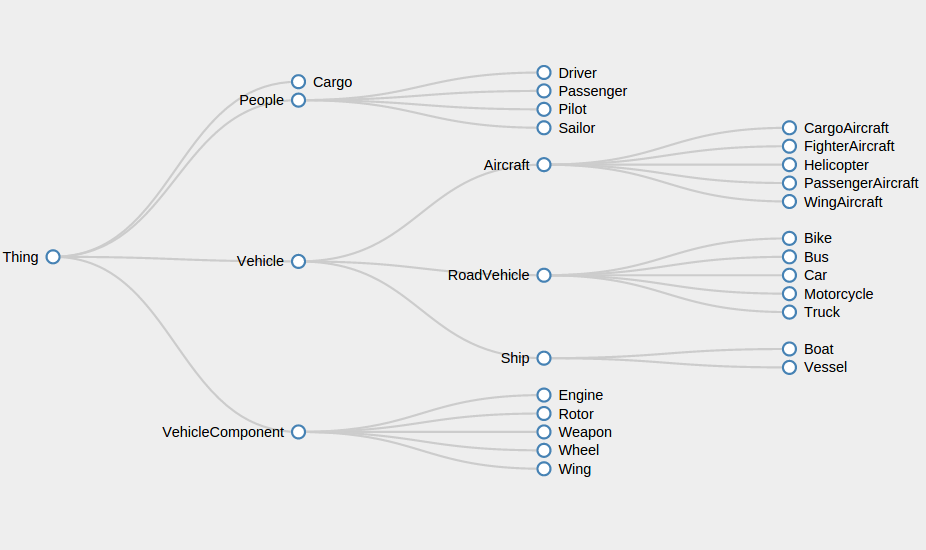
\includegraphics[width=155mm,height=105mm]{Figures/transport_cls.png}
	\caption{Các lớp trong ontology transport.owl\label{overflow}}
\end{figure}
Các lớp mở rộng ra là lớp con của lớp (node trong hình) trước nó.
\subsection{Thuộc tính đối tượng}
\begin{table}[ht!]
	\centering
\begin{tabular}{|p{3cm}|l|p{3cm}|p{3cm}|p{3cm}|}
\hline
ObjectProperty & Transitive & Domain & Range & Inverse \\ \hline
canCarry & & Vehicle & Cargo or People & canBeCarriedBy \\ \hline
isPartOf & x & Vehicle or VehicleComponent & Vehicle or VehicleComponent & hasParts \\ \hline
canBeCarriedBy & & Cargo or People & Vehicle & canCarry \\ \hline
control &  & People & Vehicle & isControlledBy \\ \hline
hasParts & x & Vehicle or VehicleComponent & Vehicle or VehicleComponent & isPartOf \\ \hline
 hasWing & & WingAircraft & Wing & \\ \hline
 hasEngine & & Vehicle & VehicleComponent & \\ \hline
 hasRotor & & Helicopter & Rotor & \\ \hline
 isControlledBy & & Vehicle & People & control \\
\hline
\end{tabular}
\caption{Bảng các thuộc tính đối tượng trong ontology transport \label{overflow}}  
\end{table}
Trong bảng 3.1 thì \textit{hasWing}, \textit{hasEngine} và \textit{hasRotor} là thuộc tính con của \textit{hasParts}.
\subsection{Thuộc tính dữ liệu}
\begin{table}[ht!]
\centering
\begin{tabular}{|l|l|l|l|}
\hline
DataProperty & Functional & Domain & Range \\ \hline
canCarryNumberOfPassenger & x & Vehicle & positiveInteger \\ \hline
canCarryTheAmountOfCargo & x & Vehicle & positiveInteger  \\ \hline
hasNumberOfSeats & x & Vehicle & positiveInteger \\ \hline
hasNumberOfWheels & x & RoadVehicle & positiveInteger  \\ \hline
canMoveOnOrIn & x & Vehicle & \{"Road" , "Sky" , "Water"\}  \\ \hline
\end{tabular}
\caption{Bảng các thuộc tính dữ liệu trong ontology transport \label{overflow}}  
\end{table}
\subsection{SWRL Rule}
Các rule trong ontology này gồm:
\begin{verbatim}
// Tàu chở hàng hóa trên 100 (đơn vị) là tàu chở hàng Vessel
Ship(?x) ^ swrlb:greaterThan(?y, 100) 
         ^ canCarryTheAmountOfCargo(?x, ?y)  -> Vessel(?x)
// Xe cộ có số chỗ ngồi lớn hơn 20 là xe bus
RoadVehicle(?x) ^ hasNumberOfSeats(?x, ?s)
                ^ swrlb:greaterThan(?s, 20) -> Bus(?x)
// Máy bay mang vũ khí là máy bay chiến đấu
Aircraft(?x) ^ canCarry(?x, ?y) ^ Weapon(?y) -> FighterAircraft(?x)
// Xe cộ có số chỗ ngồi >= 4 và <=7 là xe hơi
RoadVehicle(?x) ^ swrlb:lessThanOrEqual(?s, 7) 
^ swrlb:greaterThanOrEqual(?s, 4) ^ hasNumberOfSeats(?x, ?s) -> Car(?x)
\end{verbatim}
\subsection{Cá thể}
Lưu ý: các cá thể này đều là các cá thể có tên (NamedIndividual)
\begin{table}[ht!]
\centering
\begin{tabular}{|p{2cm}|l|p{5cm}|p{5cm}|}
\hline
Named Individual & Types & Object propety assertions & Data property assertions \\ \hline
A1 & Vehicle & \textit{canCarry} Charlie & \textit{isControlledBy} Anh \\ \hline
A2 & Vehicle & \textit{hasWing} XWing &  \\ \hline
\multirow{2}{*}{A3} & Vehicle & \textit{isControlledBy} Nguyen &  \\ 
& &\textit{hasParts} Rotor1 & \\ \hline
\multirow{2}{*}{A4} & Vehicle & \textit{isControlledBy} Nguyen &  \\ 
& &\textit{canCarry} Missile & \\ \hline
  
S1 & Vehicle &  & \textit{canMoveOnOrIn} "Water" \\ \hline
S2 & Ship &  & \textit{canCarryTheAmountOfCargo} 102 \\ \hline 
V1 & Vehicle & \textit{canCarry} Peter & \textit{canMoveOnOrIn} "Road" \\ \hline
V1 & Vehicle & \textit{canCarry} Container & \textit{canMoveOnOrIn} "Road" \\ \hline
\multirow{2}{*}{V3} & Vehicle & & \textit{hasNumberOfSeats} 6  \\
& & &  \textit{canMoveOnOrIn} "Road" \\ \hline
V4 & RoadVehicle &  & \textit{hasNumberOfSeats} 21 \\ \hline 
\end{tabular}
\caption{Bảng các cá thể trong ontology transport \label{overflow}}  
\end{table}
Ngoài ra còn có các cá thể thuộc các lớp như sau:
\begin{itemize}
\item \textbf{Passenger:} Steve, Charlie, Peter, Anh, Nguyen
\item \textbf{Pilot:} Anh, Nguyen 
\item \textbf{Weapon:} Missile, MachineGun 
\item \textbf{Wing:} XWing, YWing
\item \textbf{Cargo:} Container, SmallCargo
\end{itemize}
Trên đây, chúng em đã liệt kê ra các thực thể được chúng em tạo ra trong transport.owl và đặc điểm của chúng. Trong chương sau, chúng em sẽ trình bày tính năng phân loại dựa trên thiết kế ontology này.
\paragraph{Tổng kết} Chương này em đã trình bày qua chi tiết từng thiết kế từ giao diện phác thảo, cách tổ chức dữ liệu và xử lý sự kiện cho hệ thống và cuối cùng là thiết kế một ontology nhằm phục vụ cho quá trình phân loại khi hệ thống đã được xây dựng.
















